%\documentclass[journal=jacsat]{achemso}

\documentclass[aps,prl,reprint,amsmath,amssymb]{revtex4-1}

% define variable that compiles the main text (as opposed to SI text)
\newcommand*{\MAINTEXT}{}

%\documentclass[10pt,aps,prl,twocolumn,amsmath,amssymb,superscriptaddress,longbibliography]{revtex4-1}
%\documentclass[preprint,showpacs,preprintnumbers,amsmath,amssymb]{revtex4-1}
%\documentclass[twocolumn,showpacs,preprintnumbers,amsmath,amssymb]{revtex4}
% Some other (several out of many) possibilities
%\documentclass[preprint,aps]{revtex4}
%\documentclass[preprint,aps,draft]{revtex4}
%\documentclass[prb,amsmath,amssymb]{revtex4}% Physical Review B

\usepackage{graphicx}% Include figure files
\usepackage{dcolumn}% Align table columns on decimal point
\usepackage{bm}% bold math
\usepackage{amsmath}% bold math
\usepackage{siunitx}% si units
\usepackage{color}
\usepackage{graphicx}
%\usepackage[normalem]{ulem}
%\nofiles

\bibliographystyle{achemso}
%\bibliographystyle{naturemag}
%\bibliographystyle{abbrv}

\begin{document}

\ifdefined\MAINTEXT
\else
	\clearpage
	\widetext
	\setcounter{figure}{0}
	\setcounter{page}{1}
	\renewcommand{\thefigure}{S\arabic{figure}}
\fi

\title{
\ifdefined\MAINTEXT
\else
Supplemental Material: \\
\fi
Low-cost linear-scaling \emph{ab initio} molecular dynamics for weakly-interacting systems
%%for weakly-coupled atoms
%% for non-covalently bonded atoms
}

\author{Hayden Scheiber}
\email{hayden.scheiber@mcgill.ca}
\author{Yifei Shi}
\author{Rustam Z. Khaliullin}
\email{rustam.khaliullin@mcgill.ca}
\affiliation{Department of Chemistry, McGill University, 801 Sherbrooke St. West, Montreal, QC H3A 0B8, Canada}

\date{\today}

\ifdefined\MAINTEXT

\begin{abstract}
A density functional theory approach based on absolutely localized molecular orbitals is used in conjunction with the Langevin equation of motion to create a low-cost molecular dynamics method for weakly coupled molecular systems which retains sufficient accuracy to generate accurate dynamical properties in water. 

%The approach utilizes a systematically inaccurate potential energy surface calculation method that grows linearly in computational complexity with the size of the simulated system. 
%Systematic inaccuracies in the calculation of force using this method are balanced by a weighted version of the Langevin equation of motion. 
%The stochastic ``white noise'' of the Langevin equation acts to absorb force discontinuities while also thermostating the system to maintain the desired thermodynamic temperature. 
%In addition, we introduce a simple heuristic approach to find optimized Langevin equation parameters to use for balancing system-specific imperfect forces and maintaining correct dynamical behavior.

% We developed a linear-scaling AIMD method with low computational overhead by utilizing compact molecular orbitals strictly localized within predefined radii. High efficiency of the method is achieved without sacrificing its accuracy with a combination of two techniques: (1) on-the-fly construction of accurate localized orbitals without lengthy self-consistent optimization and (2) the unbalanced Langevin integrator that is fine-tuned to retain stable dynamics even with imperfect forces. A remarkable feature of the implemented method is that it remains efficient even for challenging condensed phase systems even if large diffuse basis sets are used. We demonstrated that, for systems well-represented by the compact orbitals (e.g. molecular systems, ionic salts), the new AIMD method enables simulations on previously inaccessible time and length scales. The first steps towards generalizing the method to more challenging systems of strongly interacting atoms (e.g. covalent crystals) will also be discussed.

\end{abstract}

\fi

\maketitle

\ifdefined\MAINTEXT

%\section{Introduction}

Since the unification of molecular dynamics and density functional theory (DFT)~\cite{a:thecpmd},
\emph{ab initio} molecular dynamics (AIMD) has become an important tool for the study of weakly bonded ensembles of molecules such as gas-phase molecular clusters, liquids, solutions, and molecular solids. %[of gas-phase molecules and condensed-phase systems.] 
Unfortunately, the computational cost of the conventional Kohn-Sham (KS) DFT grows cubically with the number of atoms, which severely limits the \emph{length scales} accessible by AIMD. %and hinders it application to large heterogeneous systems (interfaces, nuclei, defects). 
To address this issue, substantial efforts have been directed to the development of linear scaling (LS) DFT methods.

% Re-write the following section and include any recent advances
In all LS DFT methods, the \emph{delocalized} eigenstates of the effective KS Hamiltonian must be replaced with an alternative set of \emph{local} electronic descriptors
~\footnote{The delocalization of KS orbitals over all atoms is the main reason for the steep growth of the cost of KS DFT: since both the number of orbitals and the number of localization regions (e.g. atomic basis functions) increase linearly with the number of atoms, the total number of the electronic degrees of freedom grows quadratically.}. 
Most LS methods~\cite{a:linscale3,a:lee-yang-1996,a:ls-scuseria-1997,a:ls-manolopoulos-1998,a:ls-helgaker-2001,a:ls-niklasson-2003,a:curvy2,a:ls-dm-sign} explore the natural locality of the one-electron density matrix (DM). 
However, in typical DFT calculations that require diffuse basis functions, the DM approach is advantageous only for impractically large systems~\cite{a:ls-rev-1999,a:ls-dm-sign,a:almo-ls}.
Therefore, the application of DM-based LS methods have been restricted to minimal-basis tight-binding problems. 
The optimal basis variants of the DM methods~\cite{a:ls-stechel-1994,a:ls-gillan-1995,a:ls-gillan-1996,a:ls-onetep-2003, RZK-MAO} designed to rectify this issue contract large basis sets into a small number of new localized basis functions and then optimize the DM in the contracted basis. 
Although such methods have been successfully used for the evaluation of accurate DFT energies of large static systems~\cite{a:ls-onetep-2009,a:ls-conquest-2010,a:ls-onetep-2010-app1,a:ls-rev-2012} their use in AIMD is hampered by the costly optimization of both the contracted orbitals and the density matrix. 

To obviate the DM optimization, another set of electronic descriptors can be constructed by enforcing strict locality on one-electron orbitals and, necessarily, by relaxing the orthogonality constraints imposed on them. 
From the computational point of view, LS methods based on the direct optimization of such compact localized nonorthogonal orbitals~\cite{a:ls-galli-parrinello-1992,a:ls-mauri-galli-car-1993,a:ls-ordejon-1993,a:ls-mauri-galli-1994,a:ls-ordejon-1995,a:ls-kim-mauri-galli-1995,a:ls-fattebert-2004,a:ls-fattebert-2006,a:burger-yang-2008} are promising since they deal with fewer variational degrees of freedom than the DM methods. 
Unfortunately, the development of orbital-based LS methods has been all but abandoned because of the inherently difficult optimization of localized orbitals~\cite{a:ls-mauri-galli-car-1993,a:ls-ordejon-1995,a:ls-fattebert-2004,a:ls-rev-1999,a:weitao-yang-2013}. 

%RZK-important addition: we did not include a large family of the so-called fragmentation methods 
%included only those methods that attempt to construct  set 
%It is important to note all LS DFT methods reviewed above attempt to obtain the electronic description that do not construct  based on fragmentation methods that do that there  LS DFT methods the presented logical partitioning with the subsequent construction of localized MOs is a rather general approach used in a large number of electronic structure theories, which are collectively known as fragmentation methods~\cite{a:fragmentation-rev}. These methods vary greatly in how the partitioning and recombination are performed and, therefore, differ in accuracy and computational cost. We would like to emphasize that in our approach a proper quantum mechanical description of the entire system is constructed in the form of the total idempotent density matrix. This approach provides the most rigorous description of the electronic structure.

Thus, the high computational overhead of existing asymptotically linear-scaling DFT methods restrict their use in AIMD simulations to very short \emph{time scales}, systems of low dimensions, or problems that can be adequately described with minimal basis sets. 
On the length and time scales accessible in typical AIMD simulations, LS DFT cannot compete with the straightforward low-cost cubically-scaling KS DFT.

In this work, we developed a new orbital-based AIMD method that is not only linear scaling but also has a low computational overhead. 
Currently, the method is restricted to systems of small molecules that do not form strong covalent bonds with each other. 
The new AIMD method utilizes a recently developed LS DFT~\cite{a:almo-ls} based on absolutely localized molecular orbitals (\mbox{ALMOs}). 
Unlike delocalized KS orbitals, each \mbox{ALMO} has its own localization center and a predefined localization radius $R_{c}$ that typically includes nearby atoms or molecules~\cite{a:stoll,a:almo-ls}. 
In the current implementation, a localization center is a set of all local Gaussian atomic orbitals of one molecule. 
However the approach can be easily generalized to other local and nonlocal basis sets~\cite{a:ls-galli-parrinello-1992, Galerkin}. 
The key feature of ALMO DFT is that its one-electron wavefunctions are constructed in a two-step self-consistent-field (SCF) procedure~\cite{a:almo-ls} to circumvent the problem of the sluggish variational optimization emphasized above. 
In the first step, ALMOs are constrained to their localization centers~\cite{a:khal} whereas, in the second step, ALMOs are relaxed to allow delocalization onto the neighbor molecules within their localization radius $R_{c}$. 
To achieve a robust optimization in the problematic second step, it is important to keep the delocalization component of the trial wavefunction orthogonal to the fixed orbitals obtained in the first step. 
For mathematical details, see ALMO SCF method in Ref.~\citenum{a:almo-ls}.

Once the localization radius is chosen, ALMO constraint prohibits electron density transfer between distant molecules but retains all other types of interaction such as long-range electrostatic, exchange, polarization, and, if the exchange-correlation (XC) functional includes them, dispersion interactions~\cite{a:theeda}. 
Since the importance of electron transfer decays exponentially with distance, the \mbox{ALMO} approximation provides a natural and accurate representation of the electronic structure of molecular systems with just a few local variables. 
Because of the greatly reduced number of electronic descriptors and the robust optimization, the computational complexity of ALMO DFT grows linearly with the number of molecules while its computational overhead remains very low. These features make ALMO DFT a promising method to perform accurate AIMD simulations of large molecular systems.

%To decrease the cost even further, the present paper builds on the ALMO SCF method as well as other recent work involving Brownian dynamics to compensate errors in the forces~\cite{a:ls-parinello,a:2ndcpmd,a:langevin-why}. 
%We will show that our approach lowers the computation cost pre-factor for the ALMO SCF method, while maintaining LS and accuracy for calculation of dynamical properties. 
%This is done by balancing a new computationally economical but systemically inaccurate force calculation method with an optimized version of the Langevin Equation of motion. 
%We also introduce an easy to follow heuristic approach to optimize a system for generating correct dynamical behaviour.

The challenge of adopting ALMO DFT for dynamical simulations arises from the slightly nonvariational character of the localized orbitals. First, while ALMOs are variationally optimized in both SCF steps, the occupied-space projector obtained in the first step must remain fixed during the second step to ensure convergence. Second, some neglected electron transfer effects can suddenly become active in the course of a dynamical simulation when a neighboring molecule passes the localization threshold $R_{c}$. In addition to the ALMO-specific issues, the variational optimization in any AIMD methods is never truly complete and is interrupted once the norm of the gradient of the energy with respect to the variational electronic degrees of freedom drops below small but nevertheless finite convergence threshold $\epsilon_{\text{SCF}}$. While these non-SCF errors are minor and do not affect accuracy of static ALMO DFT calculations, geometry optimization, and ALMO-based Monte-Carlo simulations, they accumulate in molecular dynamics trajectories resulting in non-physical sampling and eventually disrupting them.

%For any finite value of $R_{c}$, forces are undefined at manifold of due to the discontinuous jump in potential energy when a neighboring molecule passes beyond the localization radius $R_{c}$ and is suddenly ignored in potential energy calculations. 
%Setting $R_{c}$ to larger values can reduce the magnitude of the discontinuity, but increases the computational cost as longer distance (but physically less important) interactions must be calculated. 
%As long as the discontinuity in force is small compared with the random numerical noise in the calculation, it can be safely ignored~\cite{RZK-any-references}. This means that $R_{c}$ has to be kept relatively large to maintain stable and accurate dynamics.

%While these issues can be resolved by  by increasing  to account for non-SCF forces, increasing  and decreasing While  are the known formal strategies for resolving these 

In order to maintain stable and accurate dynamics, one could use a set of strategies that includes computing the non-SCF contribution to the forces through a coupled perturbed procedure, increasing $R_{c}$, and decreasing $\epsilon_{\text{SCF}}$. %relative to the corresponding optimal values for static energy calculations or Monte-Carlo simulations. 
This however would dramatically increase the computational cost of the ALMO AIMD. %as longer-distance but physically unimportant interactions must be calculated with an additional iterative coupled perturbed solver. 
%
In this work we propose another approach, which obviates the need in a coupled-perturbed solver, allows for relaxation of the tight constraints on $R_{c}$ and $\epsilon_{\text{SCF}}$, and thus keeps the complexity and cost of simulations low. 

In our approach, the forces on atoms are calculated \emph{approximately} after the two-step ALMO SCF using a straightforward procedure that computes only the Hellmann-Feynman and Pulay components and neglects the computationally intense non-SCF component of the forces. 
The difference between these approximate ALMO forces and the \emph{reference} forces that would be obtained from perfectly converged fully-delocalized KS orbitals is $\delta f_{i\alpha}(t)$:
%
\begin{align}
\label{eq:deltaf}
f^{\text{KS}}_{i\alpha}(t) = f^{\text{ALMO}}_{i\alpha}(t) + \delta f_{i\alpha} (t),
\end{align}
%
where $\alpha$ is a Cartesian component of the force acting on atom $i$ at time $t$. $\delta f_{i\alpha} (t)$ comprises all neglected terms that originate from a finite localization radius $R_c$ and incomplete SCF optimization. 
$\delta f_{i\alpha} (t)$ can be reduced \emph{systematically} to zero by increasing $R_c$ and decreasing $\epsilon_{\text{SCF}}$. %$\epsilon_{\text{SCF}}$ is chosen such that the electronic ground state is considered sufficiently close to the Born-Oppenheimer state for values less than $\epsilon_{\text{SCF}}$.
%RZK For $\epsilon_{\text{SCF}} \leqslant 10^{-7}$~a.u. ALMO SCF is considered converged.

%The approach is inspired by ``Second Generation Car-Parinello'' MD~\cite{a:2ndcpmd} and

Our approach to compensate for the missing $\delta f_{i\alpha}(t)$ term follows the methodology that have been introduced into AIMD by Krajewski \emph{et al.}~\cite{PRB-73-041105R}, formalized by K\"uhne \emph{et al.}~\cite{a:2ndcpmd} and rationalized by Dai \emph{et al.}~\cite{a:langevin-why} before becoming informally known as the second generation Car-Parrinello molecular dynamics~\cite{doi:10.1002/wcms.1176}. 
Inspired by this method, ALMO AIMD is chosen by be governed by the Langevin equations of motion, which can be written using the unknown reference forces as:
%
\begin{align}
\label{eq:langevin}
m_i \ddot{r}_{i\alpha} = f^{\text{KS}}_{i\alpha}(t) - \gamma m_i \dot{r}_{i\alpha} + R^{\gamma}_{i\alpha} (t),
\end{align}
%
where $m_i$ is the mass of atom $i$, $r_{i\alpha}$ is its position along dimension $\alpha$, $\gamma$ is the Langevin scaling factor, and $R^{\gamma}_{i\alpha} (t)$ is stochastic force represented by a white Gaussian noise with the zero mean and the strength related to the damping term through $\gamma$:
%
\begin{align}
\label{eq:stochastic}
\langle R^{\gamma}_{i\alpha} (t) \rangle &= 0, \\
\langle R^{\gamma}_{i\alpha} (t)  R^{\gamma}_{j\beta} (t') \rangle &= 2 k_B T \gamma m_i \delta_{ij} \delta_{\alpha\beta} \delta(t-t').
\end{align}
%
This relation means that, for any value of $\gamma$, the perfectly balanced damping and stochastic terms will maintain a constant average temperature $T$ and generate the correct Maxwell-Boltzmann distribution of velocities~\cite{a:Kubo-1986,b:tuckerman-stat}. 
In the limit $\gamma \rightarrow 0$, the Newton equations of motion are recovered and the microcanonical ensemble is sampled. 
Finite values of $\gamma$ correspond to imposing canonical thermostat on the system, with larger $\gamma$ leading to more random noise in trajectories, faster equilibration but more distorted results for calculated dynamical properties. 

%It has previously been shown that Langevin dynamics can be utilized to correct inaccurate force calculations to maintain correct dynamical properties.~\cite{a:langevin-why,a:2ndcpmd,b:tuckerman-stat,a:ceriotti} 

%By utilizing Eq.\ (\ref{eq:langevin}) in conjunction with the ALMO SCF method of force calculation, we will show that discontinuity in the PES can be ignored for sufficiently large $\gamma$. 
% Perhaps this statement is not correct: Note that increasing $\gamma$ increases the sample size required to generate accurate dynamical properties, as more random Gaussian noise is introduced.

%The concept of balancing errors in force calculation with the Langevin equation can be taken even further, thereby reducing computational overhead even more. 
%%During the second step of the ALMO SCF method described above, a self-consistent variational approach is taken to converge the non-orthogonal MOs. 
%Generally, this step utilizes a iterative search function in order to reduce the absolute norm of the energy gradient to some target value $\epsilon_{\text{SCF}}$. 
%Previously, $\epsilon_{\text{SCF}}$ had to be set very small to ensure sufficient convergence of the electron structure calculations. 
%By increasing the allowable $\epsilon_{\text{SCF}}$, a great reduction in computational cost can be achieved. 
%Obviously, this introduces a significant error into the calculation of forces during each time step. 

The main assumption of ALMO AIMD is that the error in the ALMO forces is well approximated by Gaussian noise $R^{\Delta}_{i\alpha} (t)$:
%
\begin{align}
\label{eq:assumption}
\delta f_{i\alpha}(t) = R^{\Delta}_{i\alpha} (t)
\end{align}
%
that obeys
%
\begin{align}
\label{eq:stochastic2}
\langle R^{\Delta}_{i\alpha} (t) \rangle &= 0, \\
\label{eq:stochastic3}
\langle R^{\Delta}_{i\alpha} (t)  R^{\Delta}_{j\beta} (t') \rangle &= 2 k_B T \Delta m_i \delta_{ij} \delta_{\alpha\beta} \delta(t-t')
\end{align}
%
This assumption, shown below to be well justified, allows us to rewrite the Langevin equations using the ALMO forces:
%
\begin{align}
\label{eq:langevin2}
m_i \ddot{r}_{i\alpha} = f^{\text{ALMO}}_{i\alpha}(t) - \gamma m_i \dot{r}_{i\alpha} + R^{\gamma + \Delta}_{i\alpha} (t)
\end{align}
%
where the two stochastic terms are combined into one $R^{\gamma + \Delta}_{i\alpha} = R^{\gamma}_{i\alpha} + R^{\Delta}_{i\alpha}$. 
The only missing piece in the modified Langevin equation is the value of $\Delta$, which describes the strength of the newly introduced stochastic term. 
This term compensates for the imperfection of ALMO forces and is required to re-balance the damping and stochastic components in the Langevin equation and generate the correct Maxwell-Boltzmann distribution in ALMO AIMD. 

%%Note that $\Delta$ can be either positive or negative depending on the system of interest. 
%%$\Delta$ was found to be positive for all simulations considered here. %, increasing the amplitude of the effective random force on the system.

%\section{Optimizing $\Delta$}

%To correctly thermostat the system of interest, $\Delta$ needs to be reduced to zero.
%This is done by finding the value of $\Delta$ and adding a third random force term $R^{-\Delta}_{i\alpha}$ to equation \ref{eq:langevin2} which cancels out the extra forces introduced to the system by $R^{\Delta}_{i\alpha}$.
%This means that a trajectory with inaccurate forces and optimized $R^{-\Delta}_{i\alpha}$ should have no long term drift in the total energy of the system. 
%Short term energy fluctuations should be expected, and can later be ``smoothed out'' by setting $\gamma$ as needed.

(RZK the integral contains dummy index $i$ in the r.h.s.) In principle, $\Delta$ can be calculated using the integral of Eq.~(\ref{eq:stochastic3})
%
\begin{align}
\label{eq:delta}
\Delta &= (2 k_B T m_i )^{-1} \int_{-\infty}^{\infty}\langle \delta f_{i\alpha} (0)  \delta f_{i\alpha} (t) \rangle dt
\end{align}
%
if one can afford computing the reference forces $f^{\text{KS}}_{i\alpha}(t)$ (i.e. $R_c \rightarrow \infty$ and $\epsilon_{\text{SCF}} \rightarrow 0$) for a short representative AIMD trajectory (see Supplemental Material). 
In practice, we found (see results below) that this approach is not particularly accurate due to the noisy autocovariance functions (ACF) from short trajectories and perhaps because the $\delta_{ij}\delta_{\alpha\beta}$ assumption in Eq.~(\ref{eq:stochastic3}) does not strictly hold. 
Nevertheless, the ACF integral can provide a reasonable starting value of $\Delta$. 
This or, in fact, any starting value can be  rapidly fine-tuned in a series of trial-and-error short ALMO AIMD runs until the equipartition theorem is satisfied: 
%
\begin{align}
\label{eq:eqipartition}
\langle \dfrac{1}{2} m_i \dot{\bm{r}}^{2}_{i} \rangle &= \dfrac{3}{2} k_{B} T
\end{align}
%
or, in other words, until the simulation stabilizes with the correct average temperature.


%\section{Implementation}

ALMO AIMD presented here was implemented in CP2K, an open source materials modeling package~\cite{www:cp2k}. 
Accuracy and efficiency of ALMO AIMD was tested using liquid water as an example. 
This system is challenging because intermolecular electron delocalization is a critical component of hydrogen bonding and must be described correctly in approximate ALMO AIMD to reproduce static and dynamical properties of liquid water. 
%To calculate properties of water at ambient conditions, 
A periodic cell containing 125 molecules was simulated for $\SI{10}{\ps}$ at a temperature of $\SI{298}{\K}$ and a constant density of $\SI{1.006}{\g\cdot\cm^{-3}}$. 
% RZK: we do not need to specify details on gamma optimization since they are well-known.
RZK algorithm~\cite{RZK} was used to integrate the Langevin equation of motion. We found that $\gamma = \SI{e-3}{\per\fs}$ is large enough to thermostat the system on the time scale of the simulation and small enough not to significantly affect dynamical properties of liquid water.
%
In the dual-representation Gaussian and plane-wave scheme implemented in CP2K~\cite{a:quickstep}, the TZV2P basis set was used to represent molecular orbitals, and a plane-wave cutoff of $\SI{320}{Ry}$ used to represent electron density. 
The XC energy was approximated using the PBE functional~\cite{a:PBEfunctional}. 
The Brillouin zone was sampled at the $\Gamma$-point and separable norm-conserving pseudopotentials were used to describe the interactions between the valence electrons and the ionic cores~\cite{a:hgh}. 

The \emph{reference} forces were calculated with fully delocalized electrons using tightly converged, $\epsilon_{\text{SCF}}=10^{-6}$~a.u., orbital transformation (OT) method~\cite{a:ot,a:ot2}. 
In ALMO AIMD, element-specific cutoff radius for electron delocalization $R_c$ was set to 1.6 in units of the elements' van der Waals radii (vdWR). This localization radius includes approximately two coordination shells of an average water molecule and was shown to reproduce the KS reference RDF perfectly in Monte-Carlo simulations~\cite{a:almo-ls}. 
%
To measure the ability of the $R^{\Delta}$ term to compensate for imperfections in ALMO forces we varied $\epsilon_{\text{SCF}}$ between tight $10^{-6}$~a.u. and loose $10^{-2}$~a.u. 

%The computation scheme used is mostly identical to that described in the implementation section of ref.\ \citenum{a:almo-ls}. 
%at $\SI{302}{\K}$ and  --- RZK: It is customary to report TARGET temperature, not the acutal average temperature. The fact the the actual temperature deviates from the target temperature by 5 K even with perfect forces shows that our simulation is still too short.
%with the Langevin thermostat with $\gamma = \SI{e-3}{\per\fs}$. 
%All other system parameters were set identical to the ALMO system.

Even with $\epsilon_{\text{SCF}} = 10^{-2}$, we stabilized the simulation at the correct average temperature and perfect Maxwell-Boltzmann distribution (Figure~\ref{fig:dynproperties}b). $\Delta$ was initially estimated at $\SI{2e-5}{\per\fs}$ using Eq.~(\ref{eq:delta}) and then refined heuristically to $\SI{6e-5}{\per\fs}$. 
%RZK: factor of 3 bothers me. Check that this is not because we sum over 3 atoms in a molecule (or over 3 dimensions).
We found that it is easier to optimize $\Delta$ when $\gamma$ is set to zero because unnecessary stochastic noise is eliminated in the trial runs. %In theory, $\Delta$ should be independent on system size. However, we found that $\Delta$ dependents on system size due to finite size effects, which decay for increasing system size.

\begin{figure}
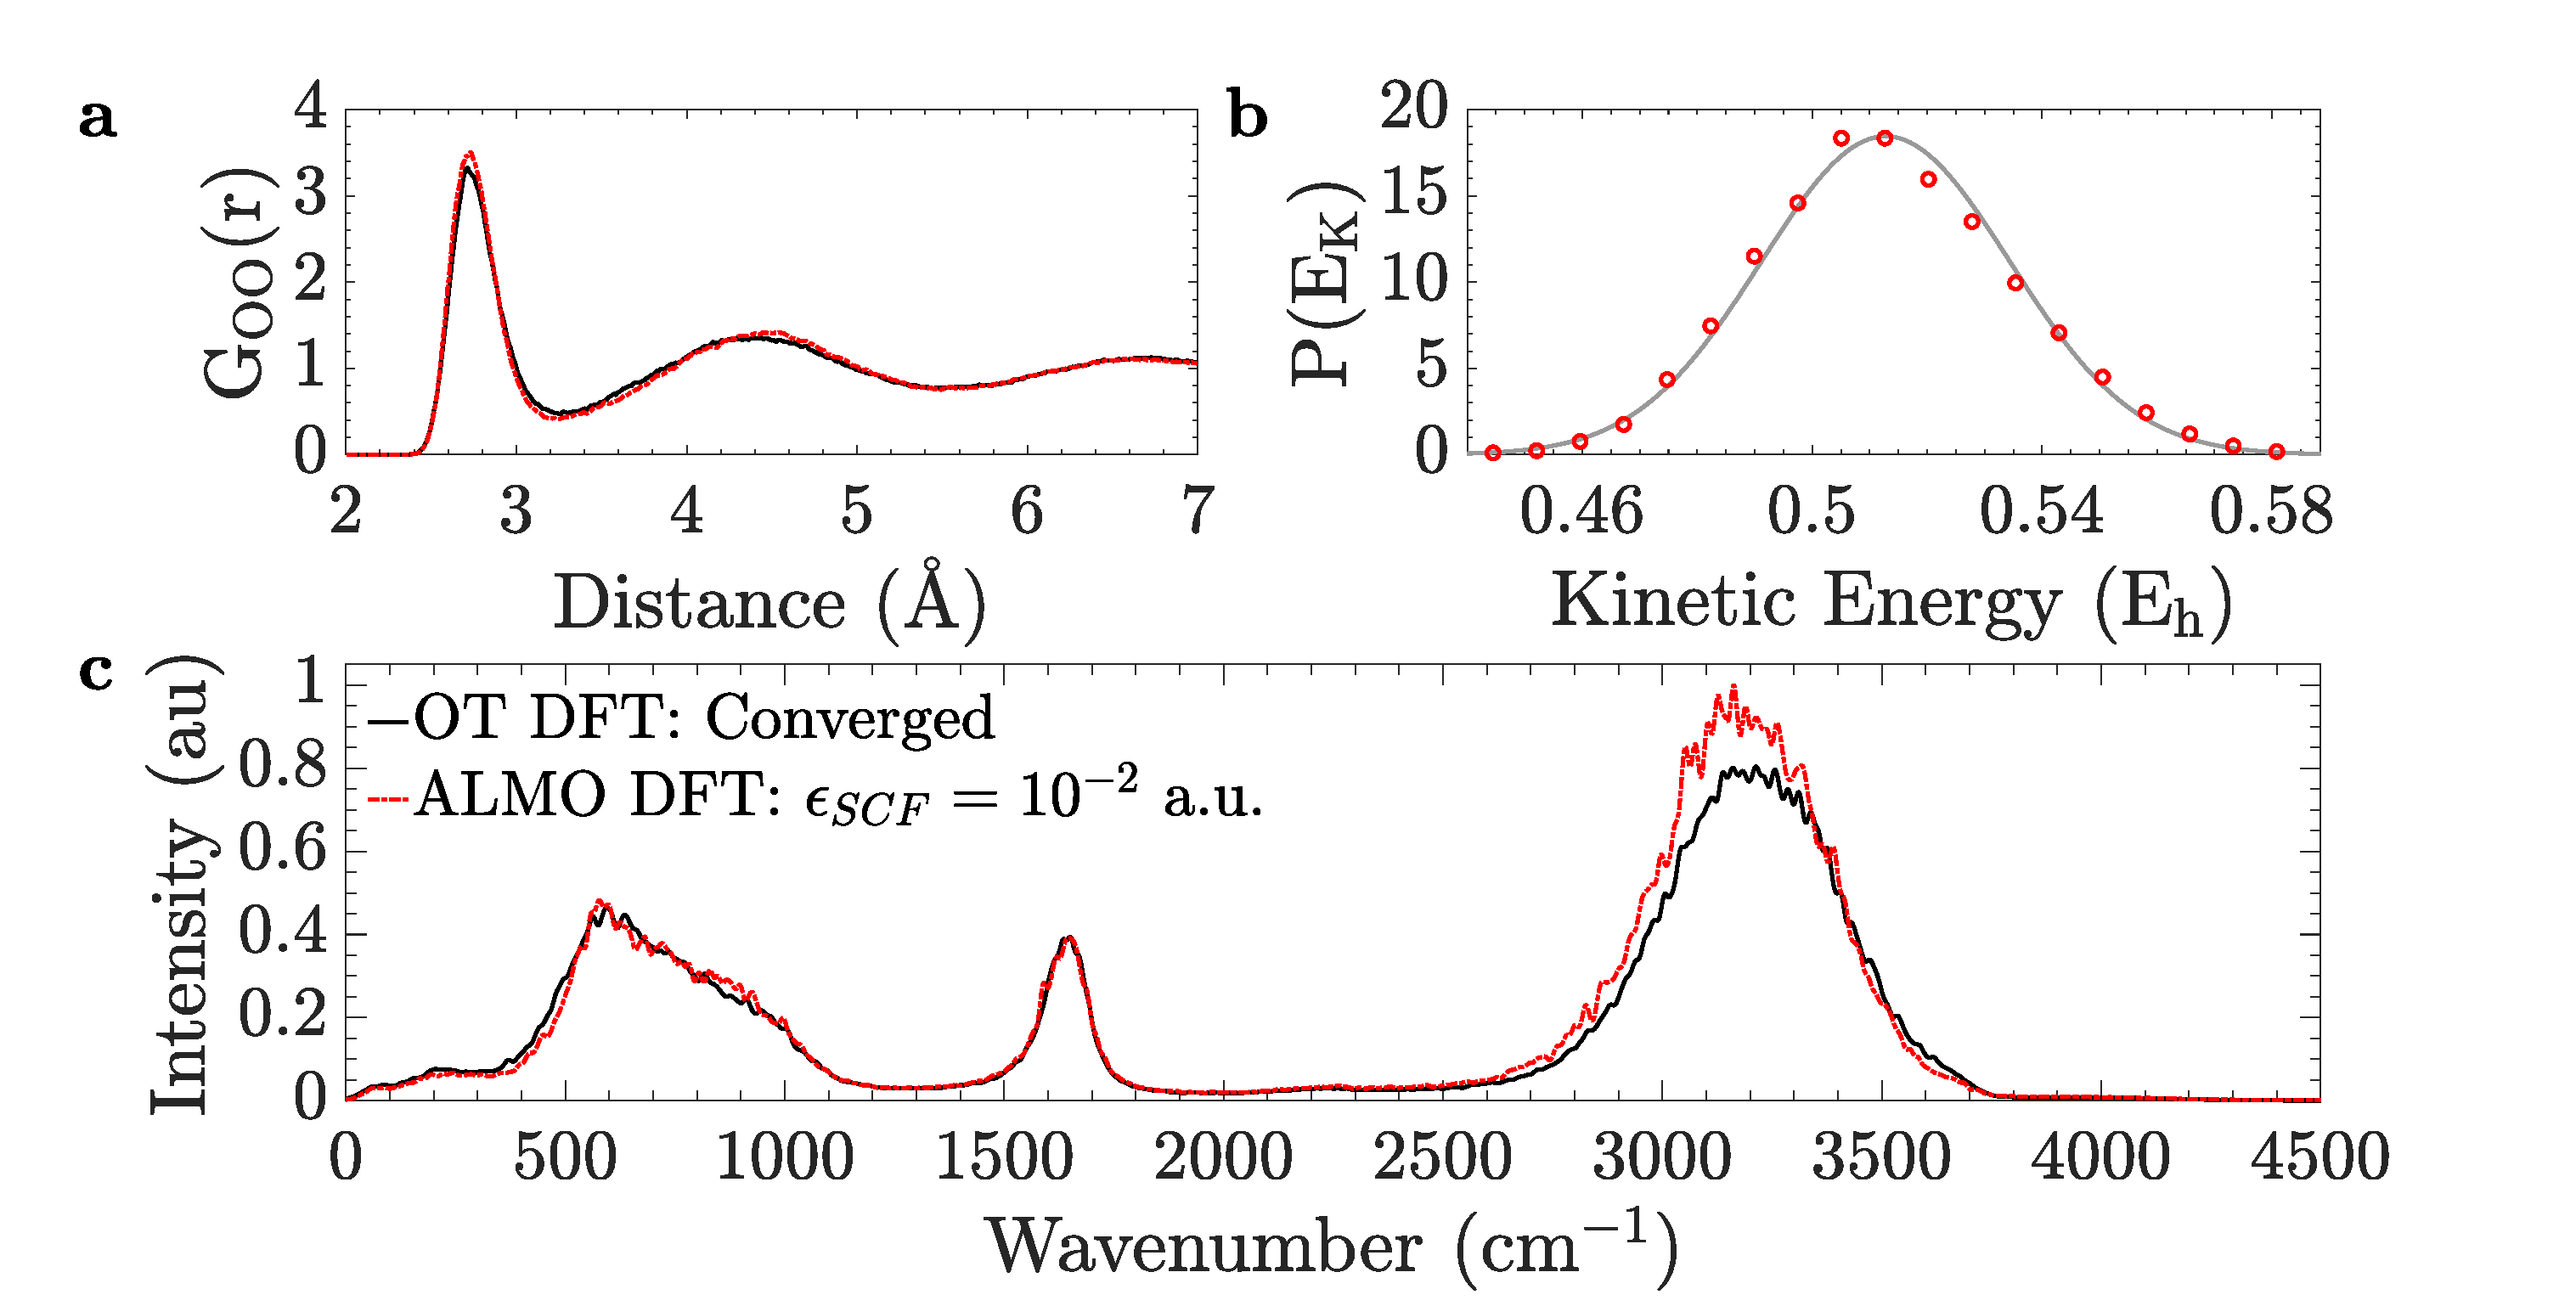
\includegraphics[trim={1.3cm 0.1cm 3.3cm 1.3cm},clip,width=8.6cm]{Dynamical_Data_Tiled.eps}
\caption{\label{fig:dynproperties} RZK:. Calculated properties of water using ALMO DFT with $\epsilon_{\text{SCF}} = 10^{-2}$~a.u. and $R_{c} = 1.6$ vdWR (red line) and fully converged OT reference (black line).
(a) radial distribution function, 
(b) kinetic energy distribution (the black curve shows the theoretical Maxwell-Boltzmann distribution), 
(c) infrared spectrum.
%Calculations were performed with the PBE $\mathrm{E_{XC}}$ functional and TZV2P basis set, using 125 water molecules for 10 ps.
}
\end{figure}

Analysis of $\delta \vec{f_{i}}(t)$ shows that the error in forces indeed resembles Gaussian white noise. The mean of the error is zero (black line in Figure~\ref{fig:randomforce}c) and the ACF decays rapidly (Figure~\ref{fig:randomforce}d) so that the error in forces can be considered uncorrelated on time scale of $\SI{50}{\fs}$. Thus the main assumptions behind our approach to ALMO AIMD are justified for liquid water. Figure~\ref{fig:randomforce}b shows that the main source of error in forces in this simulation is the loose convergence criterion and not the finite $R_c$: fully converged ALMO SCF calculations remove the rapidly oscillating component of the error. We also confirmed that the ALMO forces converge to the reference forces in the limit $R_{c} \rightarrow \infty$ (Figure~\ref{fig:forcecomp} in the Supplemental Material).

%we computed the average difference in force between fully converged Born-Oppenheimer forces and forces calculated from ALMO DFT with varying $R_{c}$. Figure \ref{fig:forcecomp} in the Supplemental Material shows that as $R_{c}$ is increased to infinity, forces converge toward the Born-Oppenheimer limit.


\begin{figure}
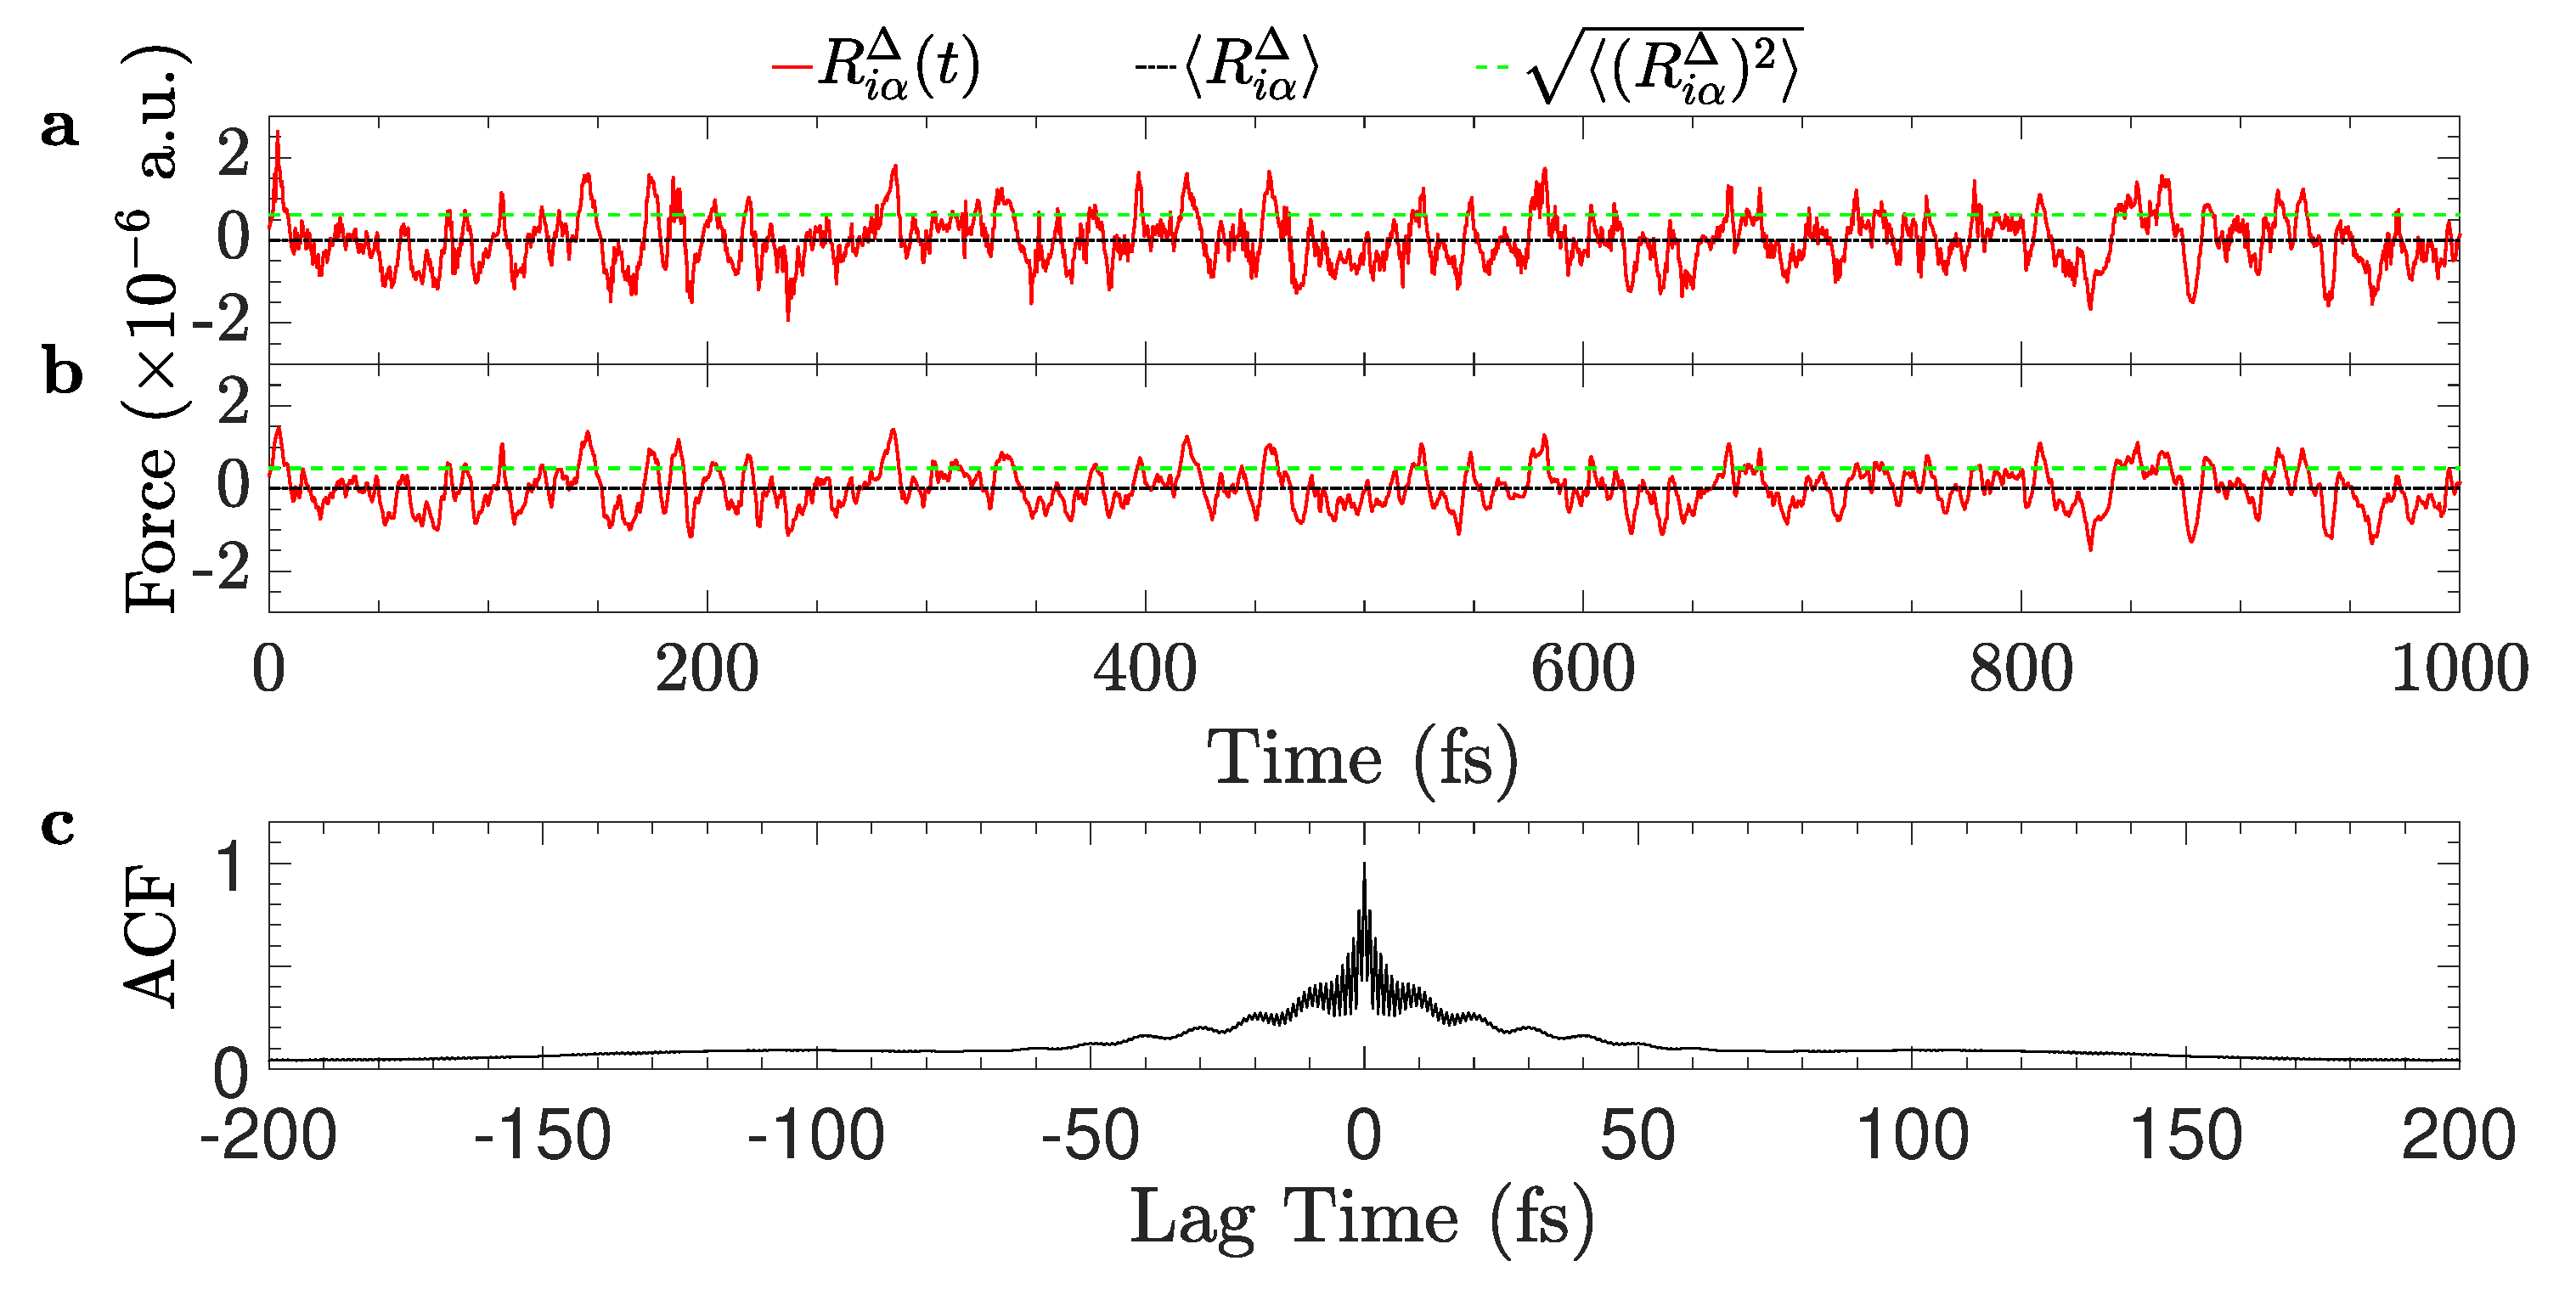
\includegraphics[trim={0.5cm 0cm 0.7cm 0.1cm},clip,width=8.6cm]{DeltaForceComparison_with_ACF.eps}
\caption{\label{fig:randomforce}  
The red line is the Euclidean norm of the instantaneous error $\langle \| \delta \vec{f_{i}}(t) \| \rangle_{i}$, the black line is the magnitude of the time average of the instantaneous error vector, and the green line is the time average of the red line. 
(a) $R_{c} = 1.6$ vdWR and $\epsilon_{\text{SCF}} = 10^{-2}$~a.u. relative to the fully converged ALMO reference, 
(b) $R_{c} = 1.6$ vdWR and fully converged ALMO SCF, relative to the fully converged OT reference, 
(c) $R_{c} = 1.6$ vdWR and $\epsilon_{\text{SCF}} = 10^{-2}$~a.u., relative to the fully converged OT reference, 
(d) Normalized ACF of the instantaneous error in panel (a) $\frac{1}{3}\langle \delta \vec{f}_i (t) \cdot \delta\vec{f}_i(t+\tau) \rangle_{it} $.
%Forces are computed with the PBE XC functional and TZV2P basis set for the configurations from a 10-ps trajectory generated with KS-based AIMD at T=298~K. 
}
\end{figure}

%\section{Accuracy}

To test the accuracy of ALMO AIMD we used trajectory analyzer TRAVIS~\cite{a:travis-main} to compute the infrared (IR) spectrum, radial distribution function (RDF), and diffusion coefficient of liquid water from both the ALMO trajectory ($\epsilon_{\text{SCF}} = 10^{-2}$~a.u. and $R_{c} = 1.6$ vdWR) and from the reference trajectory.  
The diffusion coefficients $D_{\text{OT}}=\SI{5.47e-9}{\m^{2}\per\s}$ and $D_{\text{ALMO}}=\SI{5.55E-09}{\m^{2}\per\s}$ and RDFs (Figure~\ref{fig:dynproperties}a) are in perfect agreement. The quality of the ALMO IR spectrum (Figure~\ref{fig:dynproperties}c) is good despite minor errors in the intensity of the OH stretching mode, which is sensitive to the precise positions of the centers of localized orbitals. These stringent tests show that despite noticeable errors in the ALMO forces (Figure \ref{fig:randomforce}) the compensating $R^{\Delta}$ term in the modified Langevin equation makes it possible to recover atomic dynamics properly. We would like to note that ALMO AIMD could not be stabilized with $\Delta=0$. We were not able to find any values of $\Delta$ that stabilize trajectories generated using perturbative versions of ALMO DFT~\cite{a:almo-ls}.

%\section{Speed}

%RZK Simulations for timing benchmarks were run for ten time steps, which is sufficient for convergence of wavefunctions from an initial guess.

To demonstrate the computational advantage of ALMO AIMD, we compared the average wall-time per MD step over 10 time steps for a variety of methods in Figure \ref{fig:strongscaling_log}.
In addition to the fully converged OT reference, we included timing for the second generation Car-Parrinello method, which decreases computational prefactor of the cubically scaling OT method~\cite{a:2ndcpmd}.
As expected ALMO methods show clear LS behavior for all values of $\epsilon_{\text{SCF}}$ even for medium-size systems. 
%OT SCF scales approximately cubically, as expected.
For liquid water, strict localization of molecular orbitals makes ALMO AIMD faster than the second-generation Car-Parinello for larger than 256 molecules. It is important to emphasize that comparison is performed for a three-dimensional condensed phase system described with a large diffuse basis set -- a particularly challenging case for LS methods.

\begin{figure}
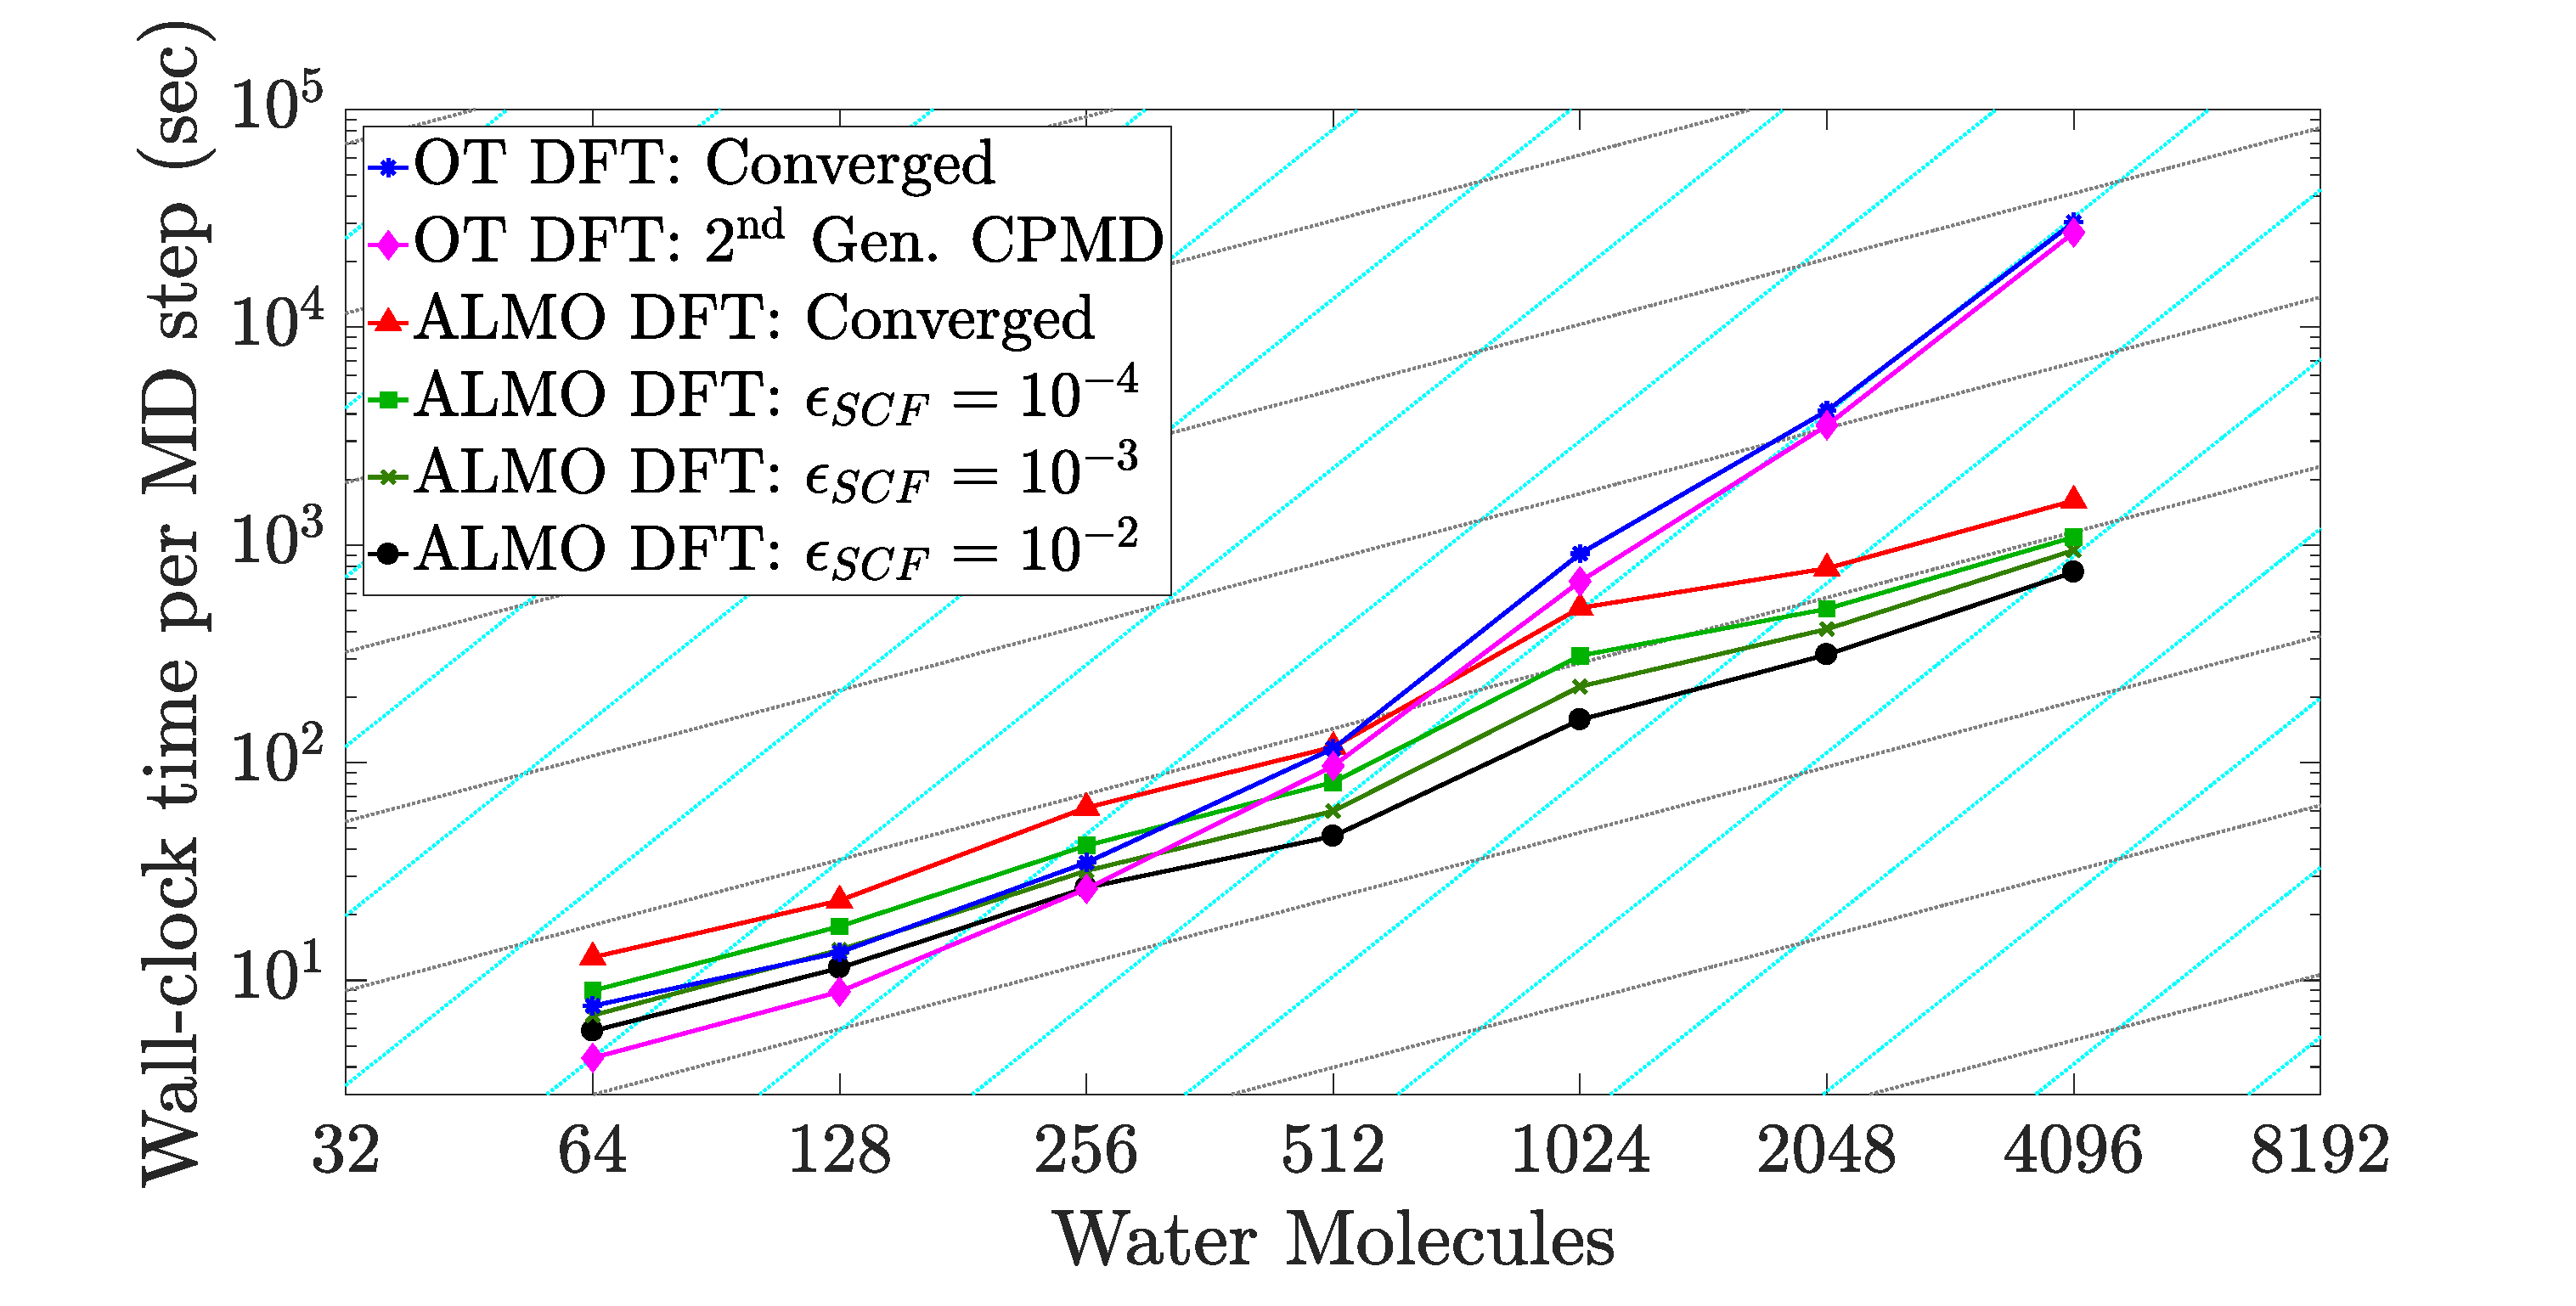
\includegraphics[trim={2.5cm 0.5cm 3.4cm 0.1cm},clip,width=8.6cm]{strongscaling_log.eps}
\caption{\label{fig:strongscaling_log} Timing benchmarks for PBE/TZV2P simulations of liquid water on 256 compute cores. 
%Logscale plots which show the asymptotic LS behaviour of ALMO methods for liquid water at 298 K.
%Compared with the orbital transformation using fully converged SCF and second generation Car-Parinello force calculation methods.~\cite{a:ot,a:ot2,a:2ndcpmd}
For ALMO methods, $R_{c} = 1.6$ vdWR. 
Cyan lines represent perfect cubic scaling, whereas gray lines represent perfect linear scaling. 
%RZK: On figure remove 'DFT', 'Wall-clock time' -> 'Wall time'
}
\end{figure}

Weak scaling benchmarks show (Figure \ref{fig:weakscaling}) that computation with localized orbitals is naturally suited for parallel execution and that the computational cost of our implementation grows linearly for a wide range of compute cores. 
It also demonstrates that the range of routine AIMD simulations can be extended from $\sim 10^3$ to $\sim 10^4$ atoms making completely new phenomena such as dynamics on interfaces and nucleation processes accessible on HPC platforms today. 
%We also show that systems as large as 8192 molecules can be simulated for 10,000 MD steps in under a month using this method.
In fact, we were able to successfully simulate systems as large as 32768 water molecules within reasonable wall-clock time using only moderate number of compute cores (Figure \ref{fig:weakscaling}) -- unprecedented feat for AIMD considering that accurate molecular orbitals and the idempotent DM are computed on each step.


\begin{figure}
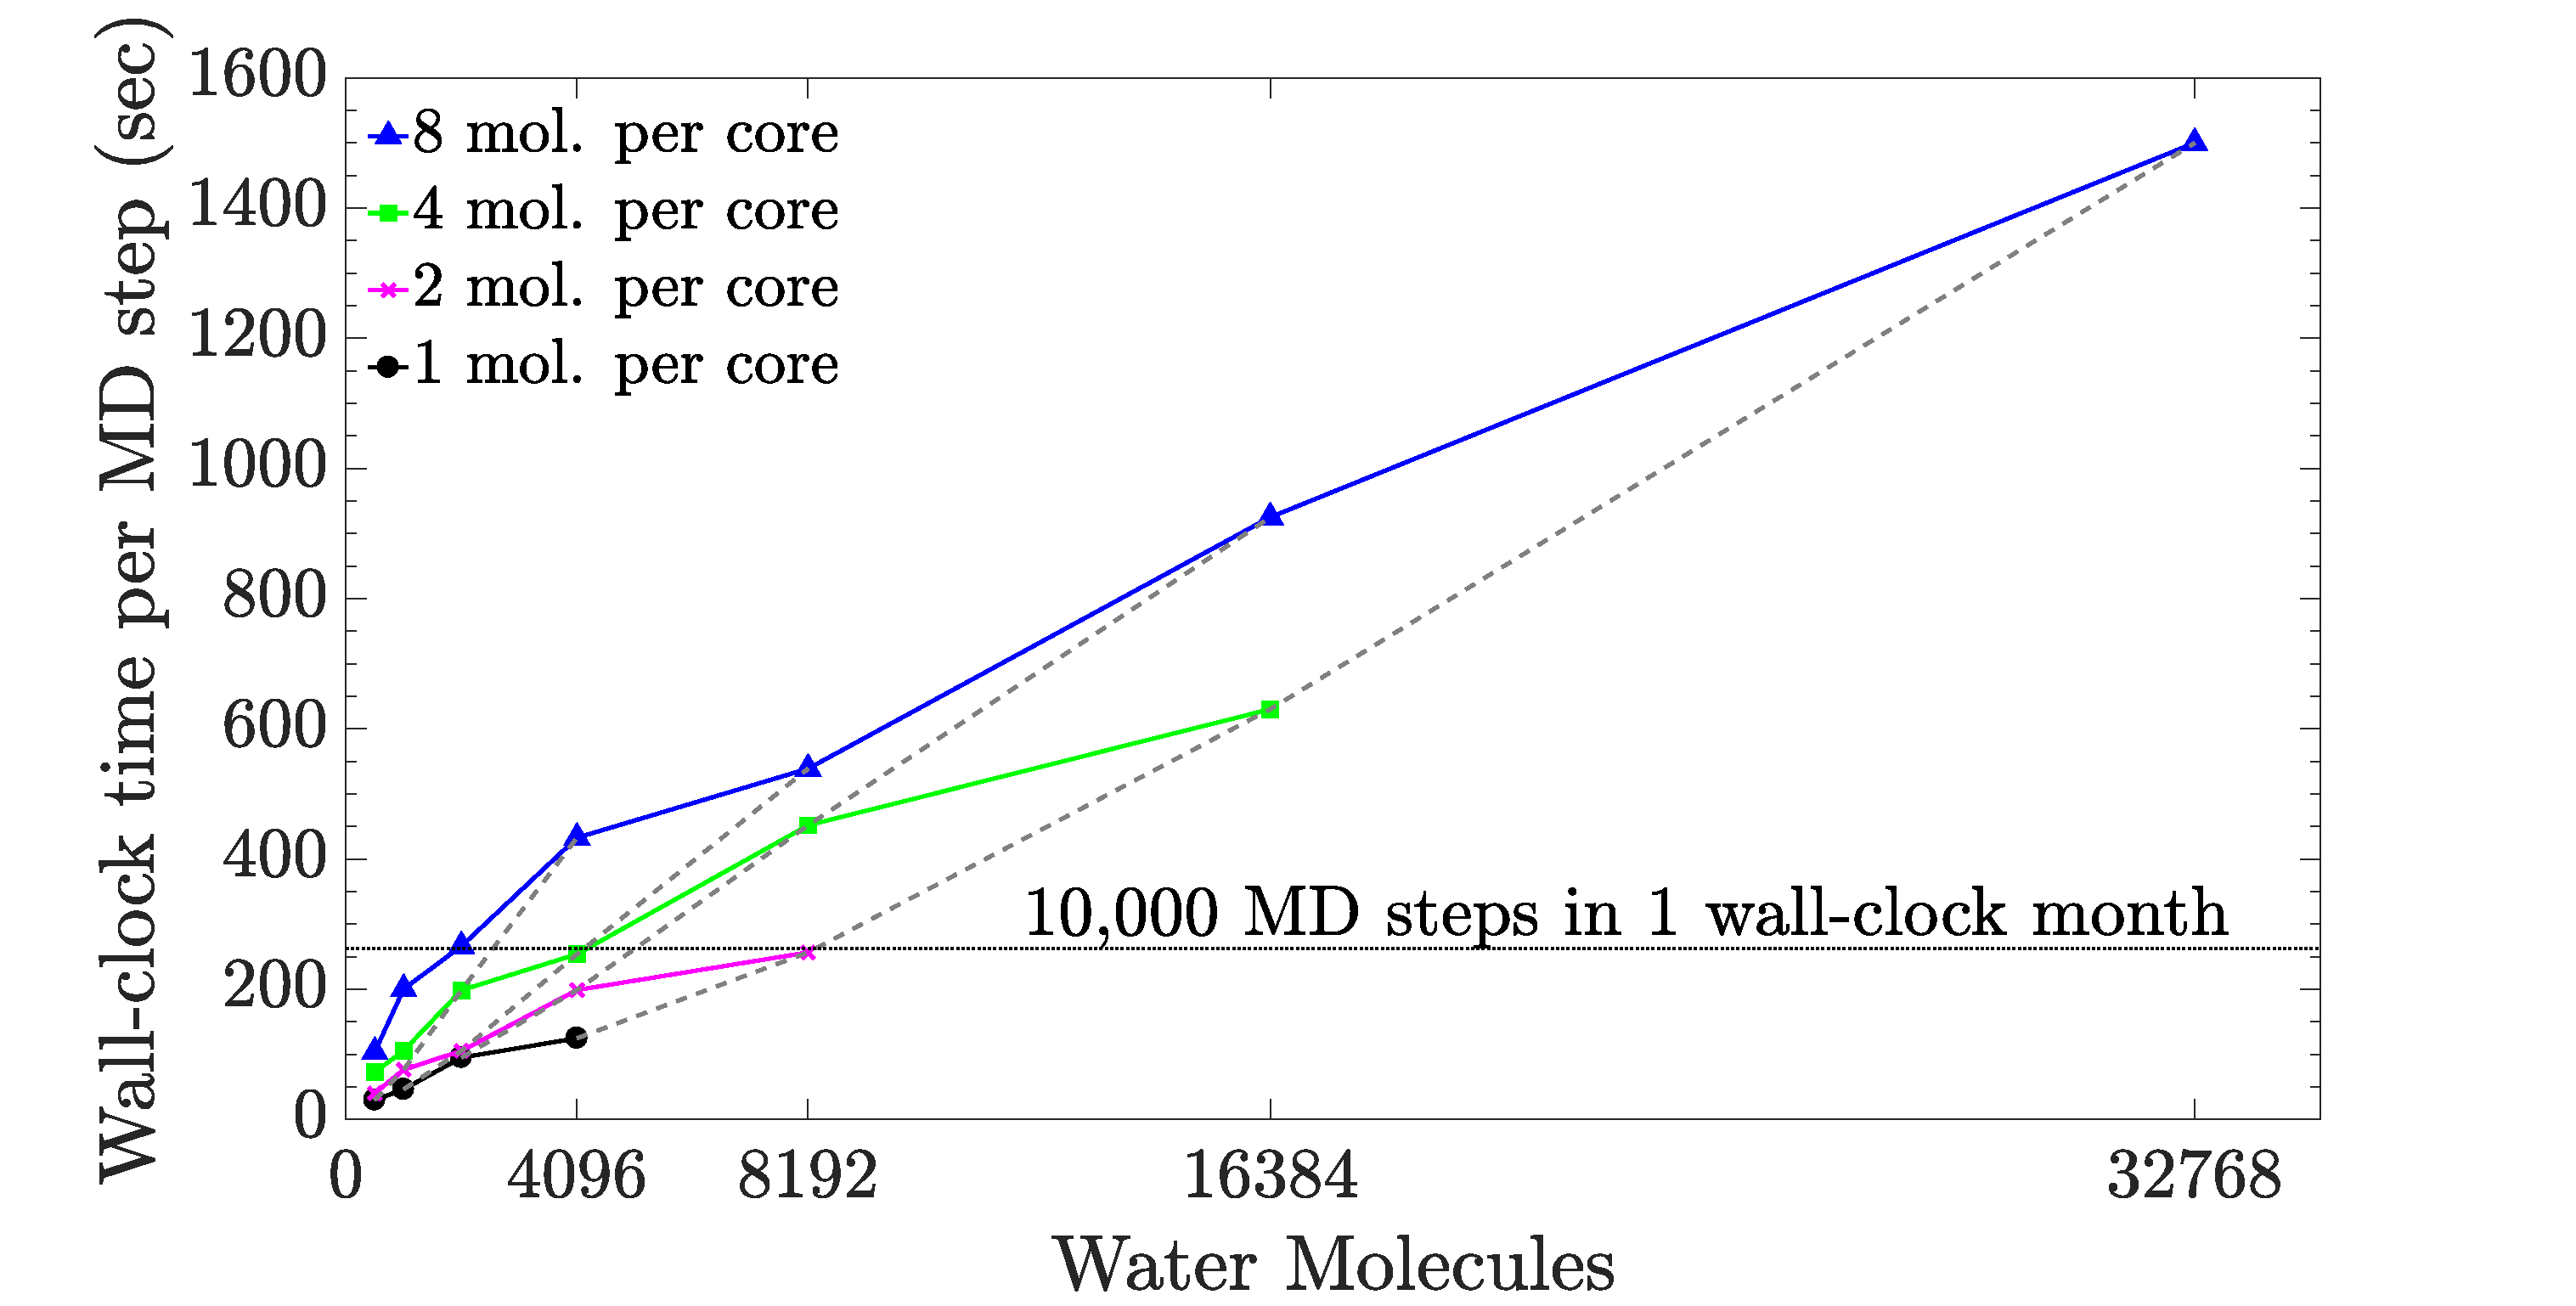
\includegraphics[trim={1.6cm 0cm 4.7cm 0cm},clip,width=8.6cm]{weakscaling.eps}
\caption{\label{fig:weakscaling} Weak scalability benchmarks for PBE/TZV2P ALMO AIMD with  $R_{c} = 1.6$ vdWR and $\epsilon_{\text{SCF}} = 10^{-2}$~a.u. 
Dashed gray lines connect systems simulated using the same number of compute cores to confirm LS behavior. %over a range of configurations.
The horizontal line corresponds to 10,000 AIMD steps in one wall month and shows a upper-bound guideline for practical AIMD.
%RZK: On figure 'Wall-clock time' -> 'Wall time', legend - increase font size, decrease the height of the figure(the y-axis label is now shorter)
}
\end{figure}

%\section{Conclusions} 

RZK: systematically improvable approximation to DFT-based AIMD.
In this article we have clearly demonstrated the utility of ALMO DFT methods, especially when combined with the Langevin Equation of motion.
ALMO DFT methods are a powerful class of AIMD electronic structure determination techniques capable of efficiently calculating forces for weakly coupled molecular systems.
It's clear that forces calculated by ALMO DFT can be tuned as accurately as required by the user, up to the Born-Oppenheimer limit.
Indeed, the ALMO DFT technique highlighted in this article has been shown to be capable of producing potential energy surfaces extremely efficiently for medium to large systems with only a minimal drop in the accuracy of calculated bulk system properties.
We have also shown that due to its linear scaling nature, the ALMO DFT technique can be pushed to simulate enormous chemical systems accurately in remarkably short calculation times.

%Using liquid water as an example, we demonstrate that the new AIMD methodology enables computational studies of molecular systems on previously inaccessible time and length scales. 

%To summarize, a low-cost linear-scaling AIMD method for weakly-interacting molecular systems was developed by utilizing compact molecular orbitals strictly localized within predefined radii. High efficiency of the method is achieved without sacrificing its accuracy with a combination of two techniques: (1) on-the-fly construction of accurate localized orbitals without lengthy self-consistent optimization and (2) a modified Langevin equation that is fine-tuned to retain stable dynamics even with imperfect forces. A remarkable feature of the implemented method is that it remains efficient for challenging condensed phase systems, even with diffuse atom-centered basis sets. Using liquid water as an example, it is demonstrated that the new AIMD method enables simulations of molecular systems on previously inaccessible time and length scales. 

Generalization of the method to more challenging systems of strongly interacting atoms such as covalent crystals is underway.

\textbf{Acknowledgments.} The research was funded by the Natural Sciences and Engineering Research Council of Canada through the Discovery Grant. The authors are grateful to Compute Canada and McGill HPC Centre for computer time.

\bibliography{almo-langevin}

\else

%\section{Procedure to estimate the value of $\Delta$}
%
%Another approach based on Eq. (\ref{eq:assumption}) can be used to find $\Delta$ within an order of magnitude if one can afford computing tightly converged SCF forces for a short MD trajectory. 
%First, run the simulation with $\Delta = 0$ and converged SCF forces. 
%Second, compute approximate forces for snapshots along the trajectory and calculate the random term $R^{\Delta}_{i\alpha} (t)$ using Eq.\ \ref{eq:assumption}. 
%Third, calculate the autocovariance function (ACF) of the noise $\text{ACF}(t) = \langle R^{\Delta}_{i\alpha} (0)  R^{\Delta}_{i\alpha} (t) \rangle$, which should be sharply peaked around zero lag time if our assumption is correct. 
%Finally, integrate Eq.(\ref{eq:stochastic3}) to obtain the following expression for $\Delta$.
%%
%\begin{align}
%\label{eq:delta}
%\Delta &= (2 k_B T m_i )^{-1} \int_{-\infty}^{\infty}\langle R^{\Delta}_{i\alpha} (0)  R^{\Delta}_{i\alpha} (t) \rangle dt
%\end{align}
%%
%In other words, we use the integral of the ACF to estimate the strength of the random force. 

\begin{figure}[!htb]
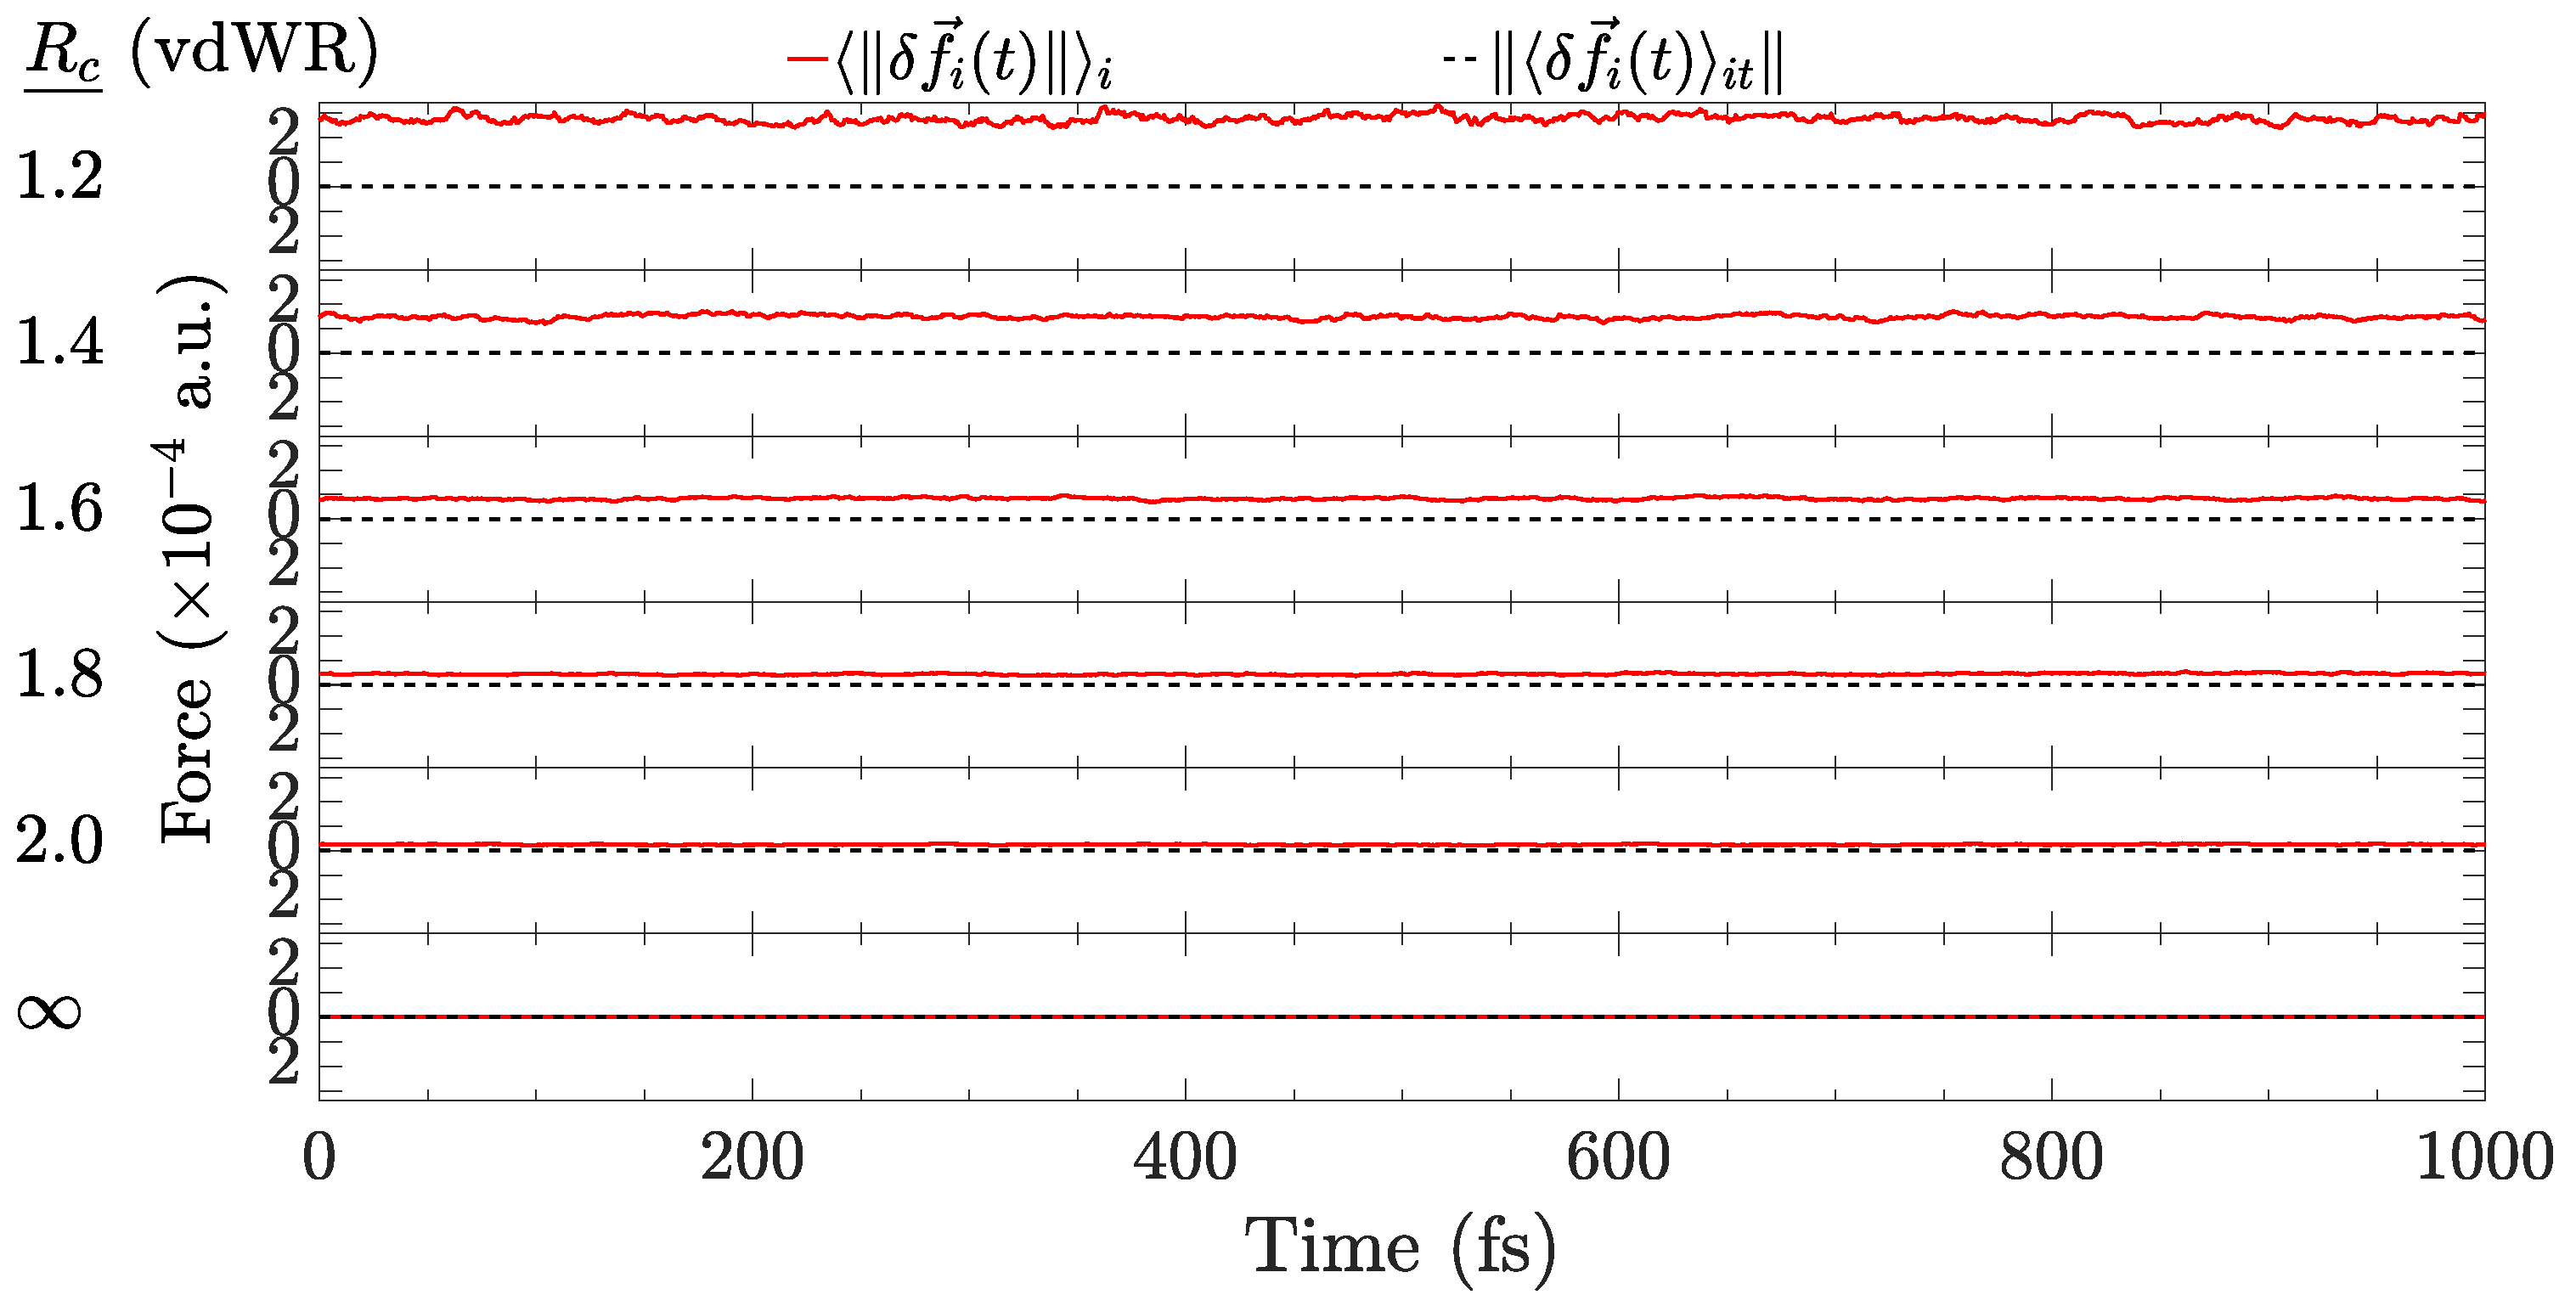
\includegraphics[trim={0cm 0cm 0.1cm 0.1cm},clip,width=\textwidth]{DeltaForceComparison_ALMO_SCF.eps}
\caption{\label{fig:forcecomp} Dependence of the Euclidean norm of the instantaneous error $\langle \| \delta \vec{f_{i}}(t) \| \rangle_{i}$ (red line) on the ALMO localization radius $R_c$ expressed in units of atomic van der Waals radii. Black line is the magnitude of the time average of the instantaneous error vector. %calculated as the average difference between fully converged Born-Oppenheimer forces and fully converged ALMO DFT forces, averaged over all dimensions and all molecules for each time step. 
Forces are computed with the PBE XC functional, TZV2P basis set, and $\epsilon_{\text{SCF}} = 10^{-7}$~a.u. for the configurations from a 10-ps trajectory generated with KS-based AIMD at T=298~K.}
\end{figure}

%\begin{figure}[!htb]
%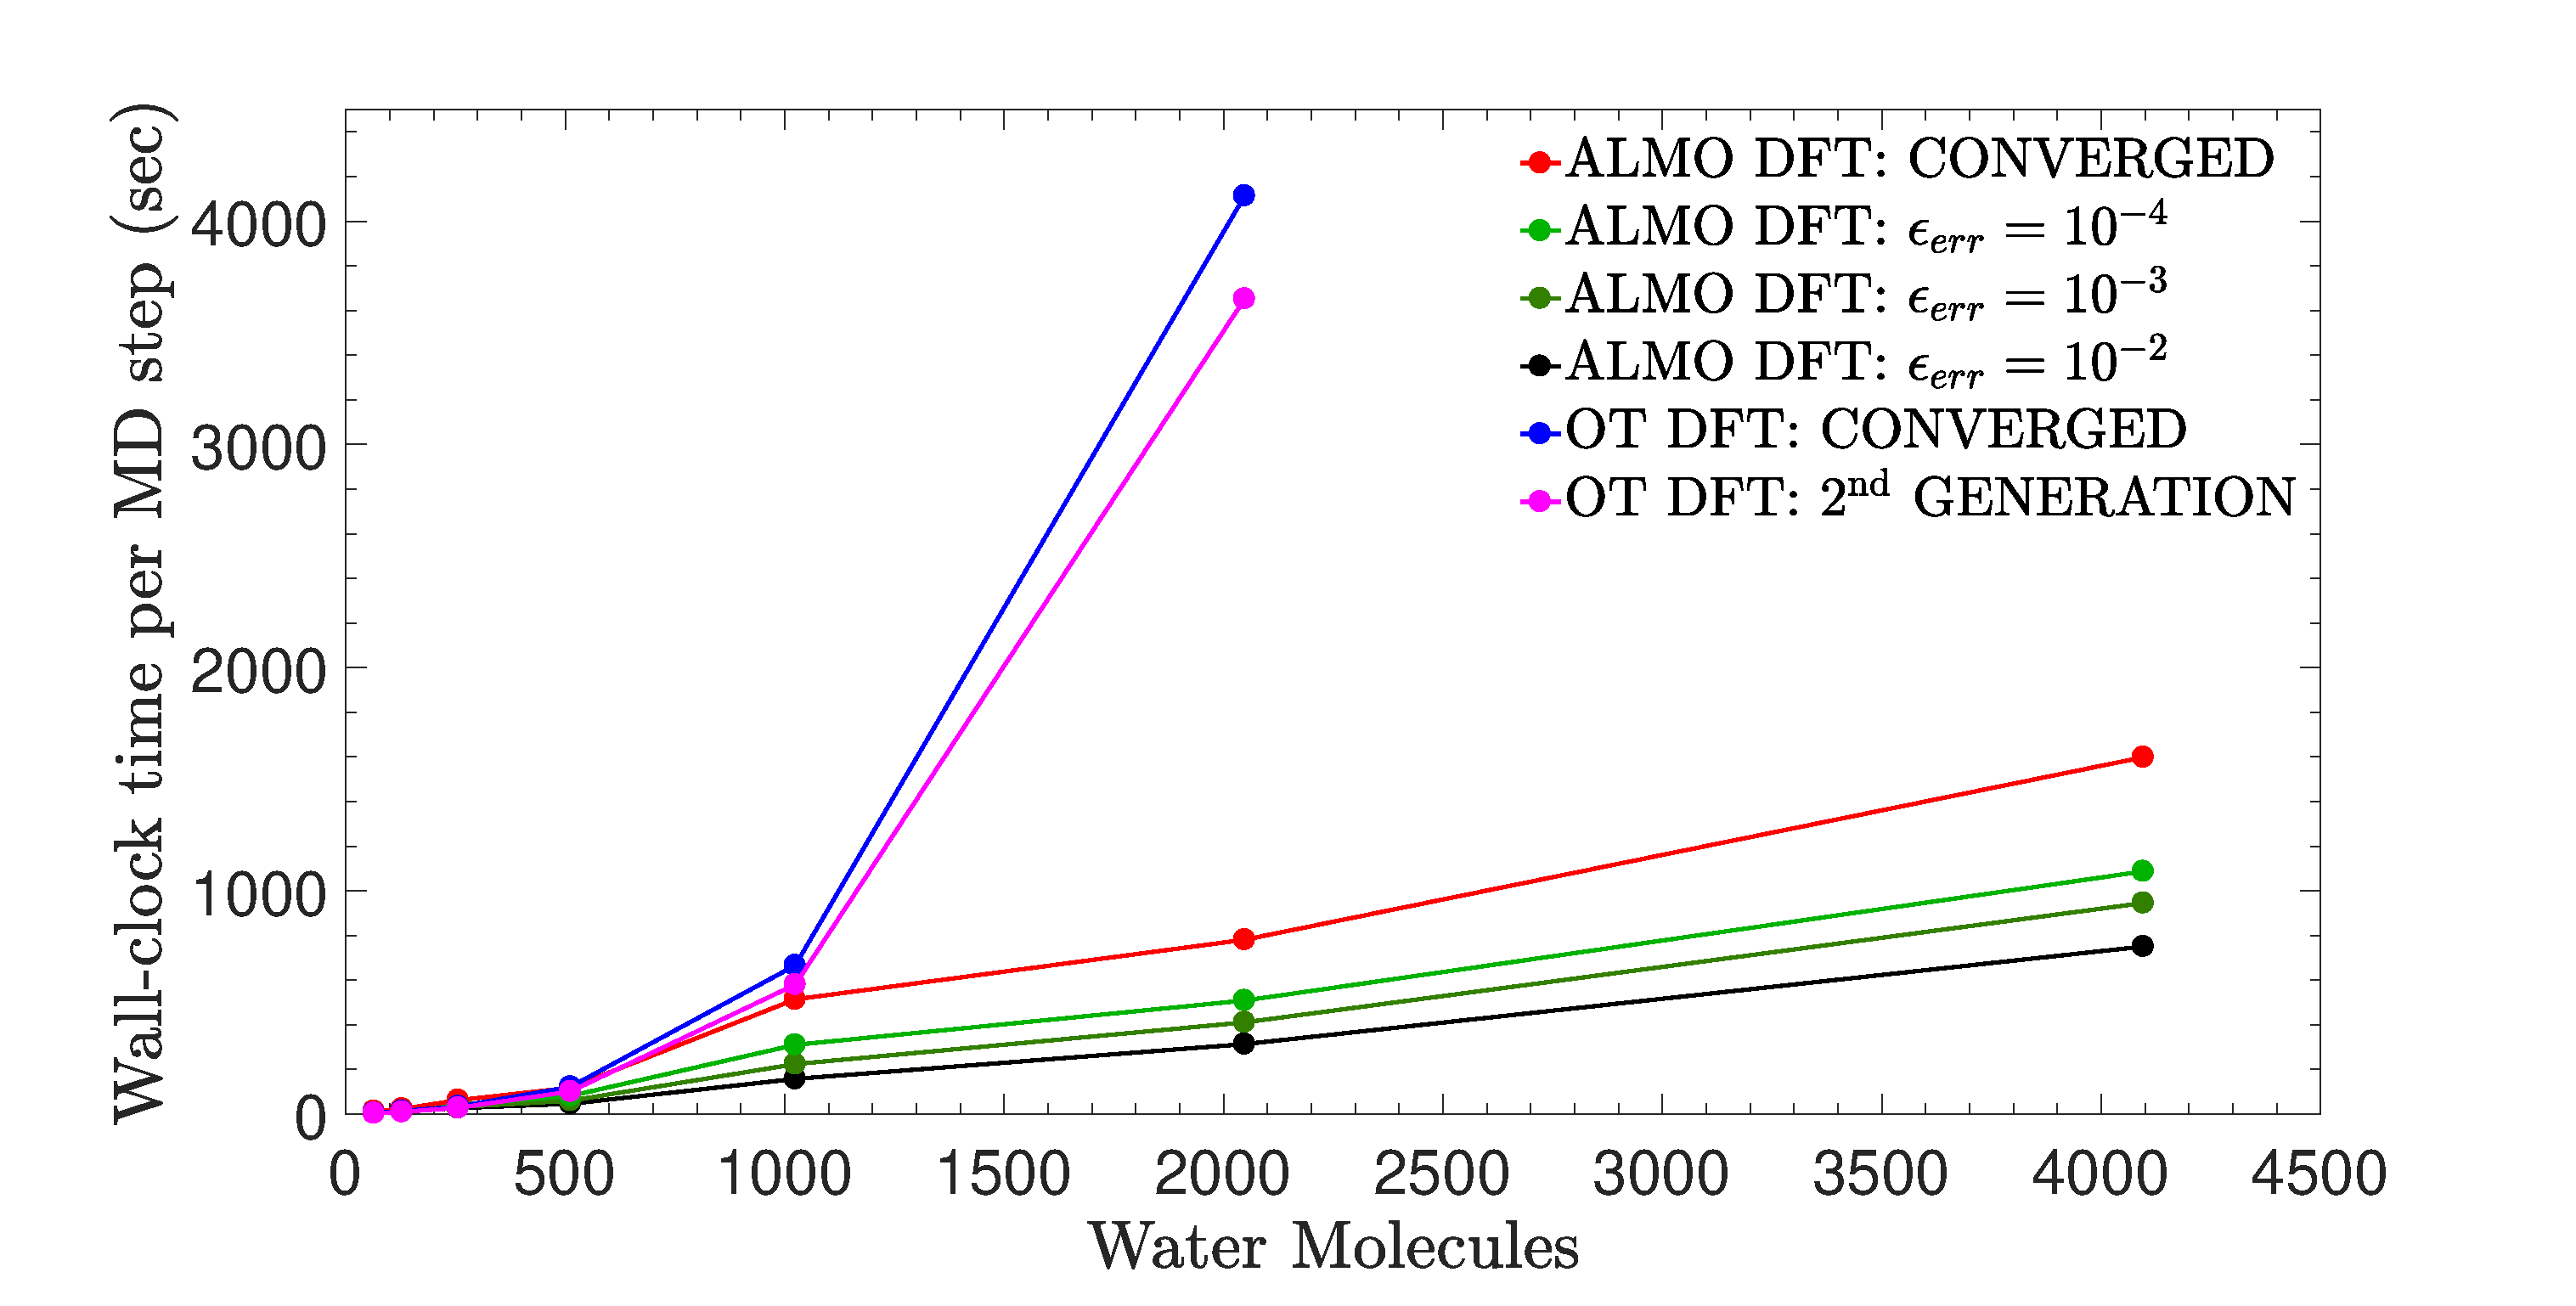
\includegraphics[trim={1.7cm 0.5cm 3.3cm 0.1cm},clip,width=\textwidth]{strongscaling_linear.eps}
%\caption{\label{fig:strongscaling_linear} Linear plots showing LS behaviour of all ALMO methods for liquid water at 298 K. 
%Calculations were performed with the PBE $\mathrm{E_{XC}}$ functional and TZV2P basis set, averaged over 10 MD steps. 
%The localization radius was set to $R_{c} = 1.6$ vdWR and $\epsilon_{\text{SCF}} = 10^{-2}$~a.u.}
%\end{figure}

%\begin{figure}[!htb]
%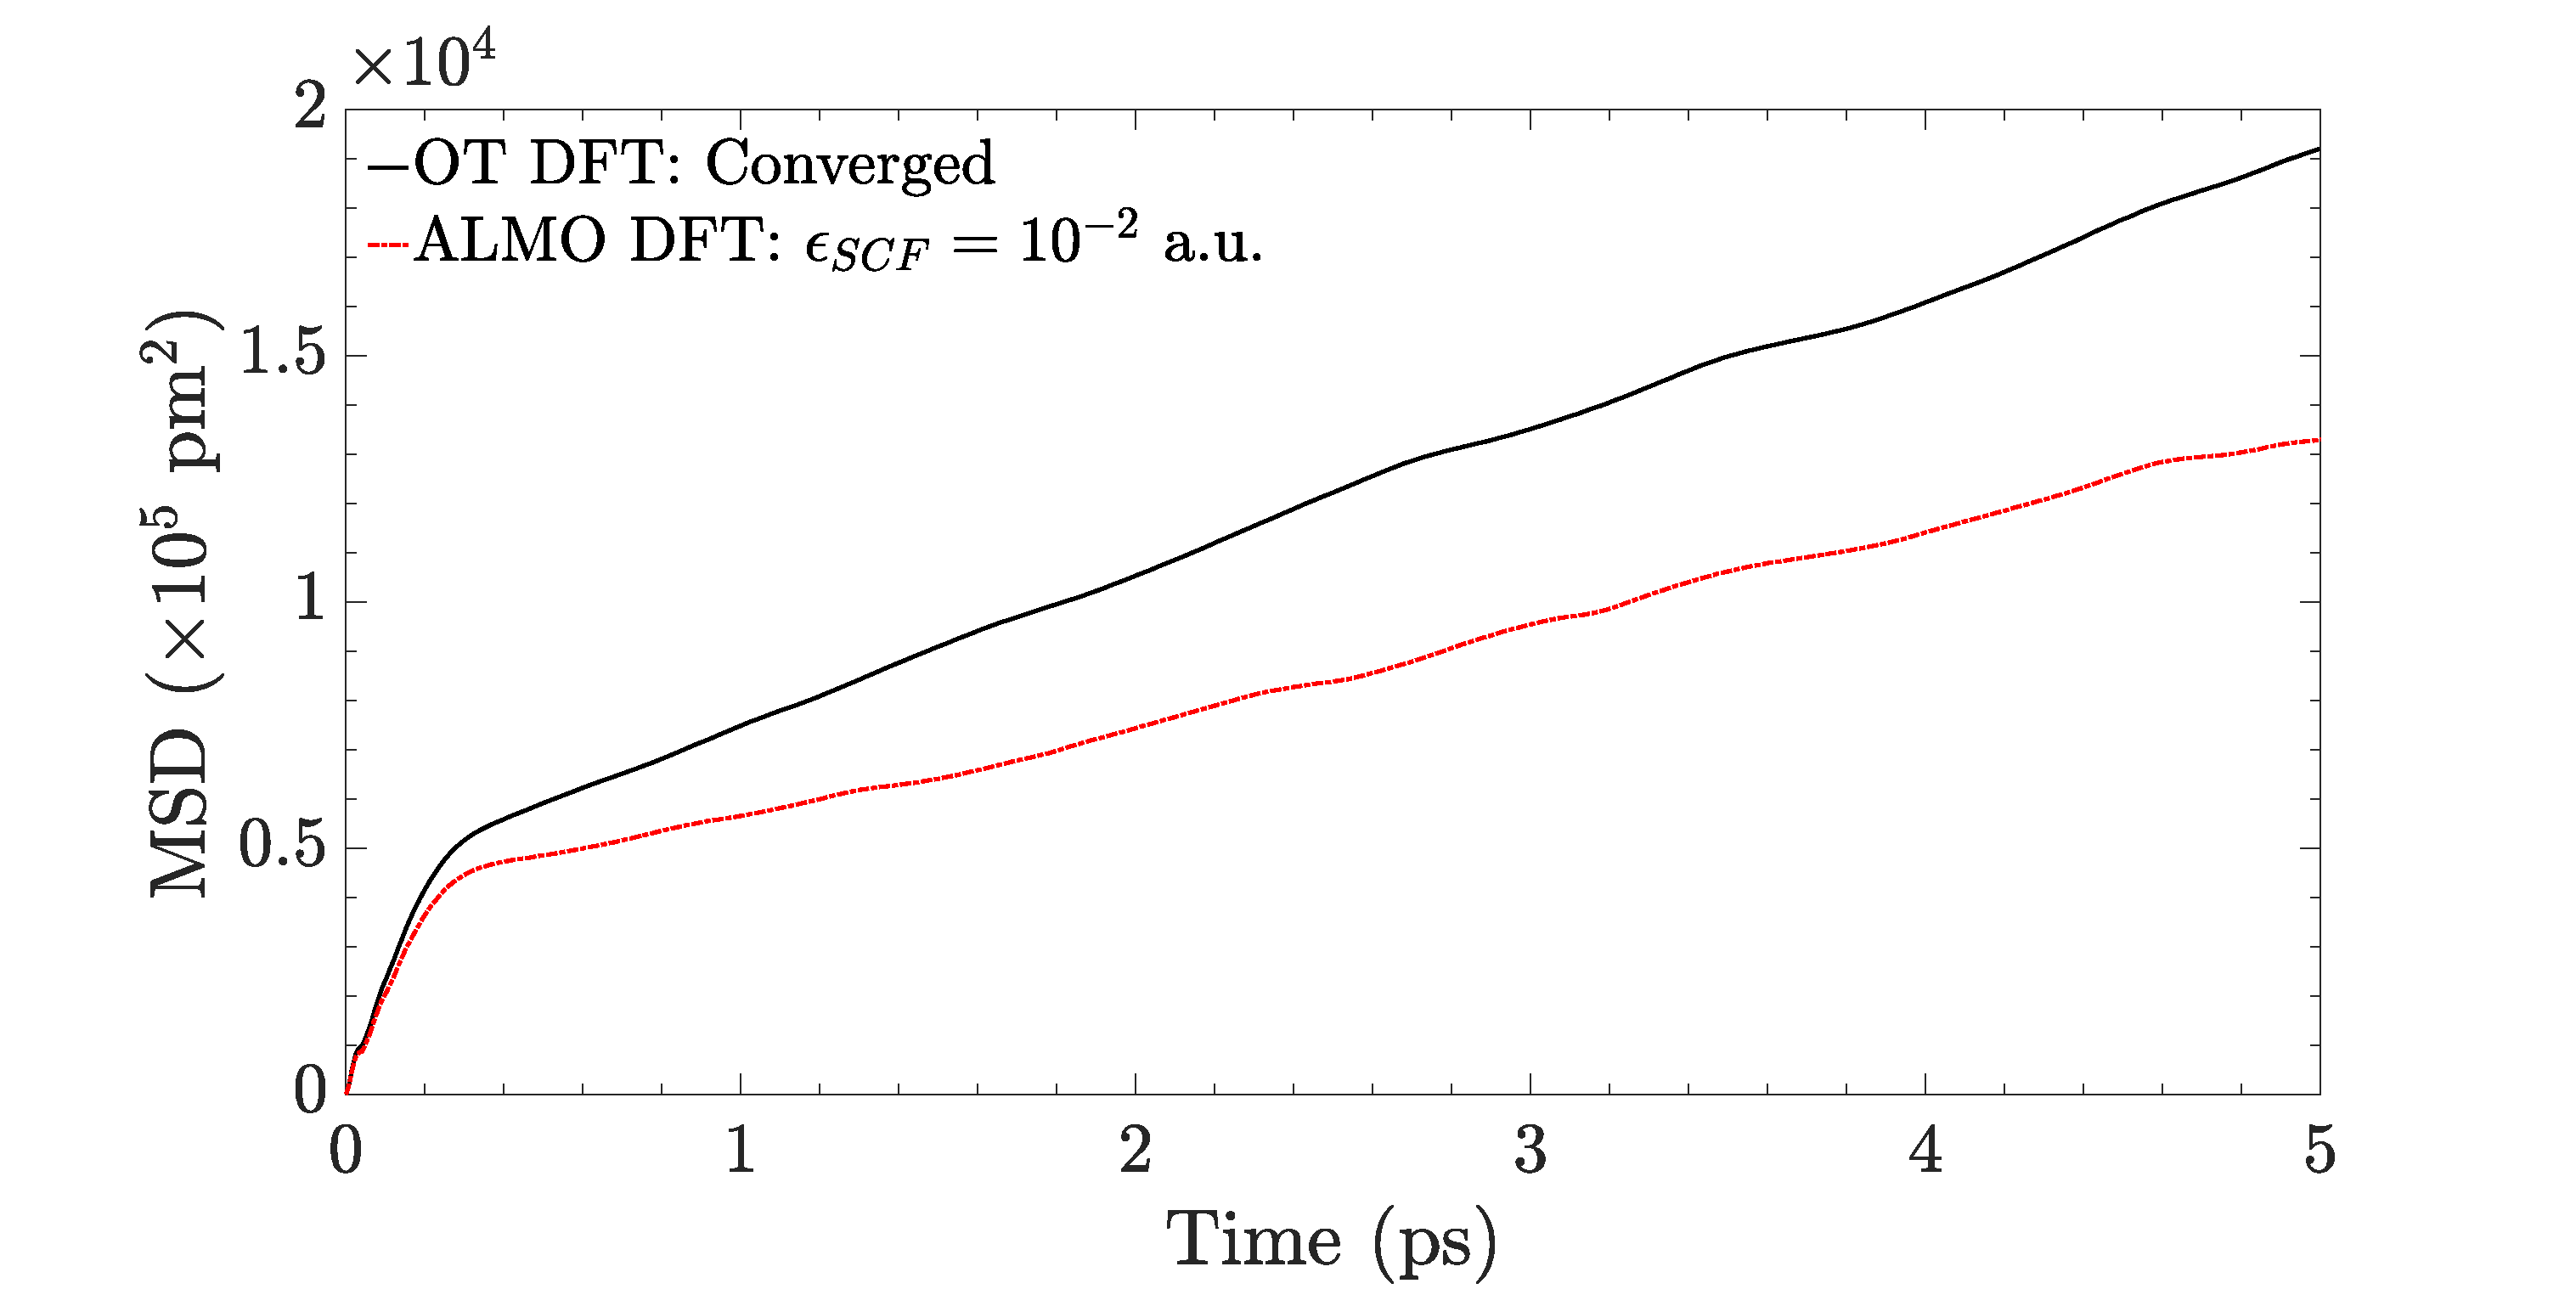
\includegraphics[trim={2.5cm 0.2cm 4.5cm 1.2cm},clip,width=\textwidth]{Diffusion_Comparison.eps}
%\caption{\label{fig:diffusion} Calculated mean-squared displacement function of water using ALMO DFT with $\epsilon_{\text{SCF}} = 10^{-2}$~a.u. and $R_{c} = 1.6$ vdWR.
%Compared with equivalent MD run using OT DFT as a reference.
%Calculations were performed at 298 K with the PBE $\mathrm{E_{XC}}$ functional and TZV2P basis set, using 125 water molecules for 10 ps.}
%\end{figure}

\fi % Manuscript <-> SI switch

\end{document}
